\begin{figure}[htbp]
	\centering
    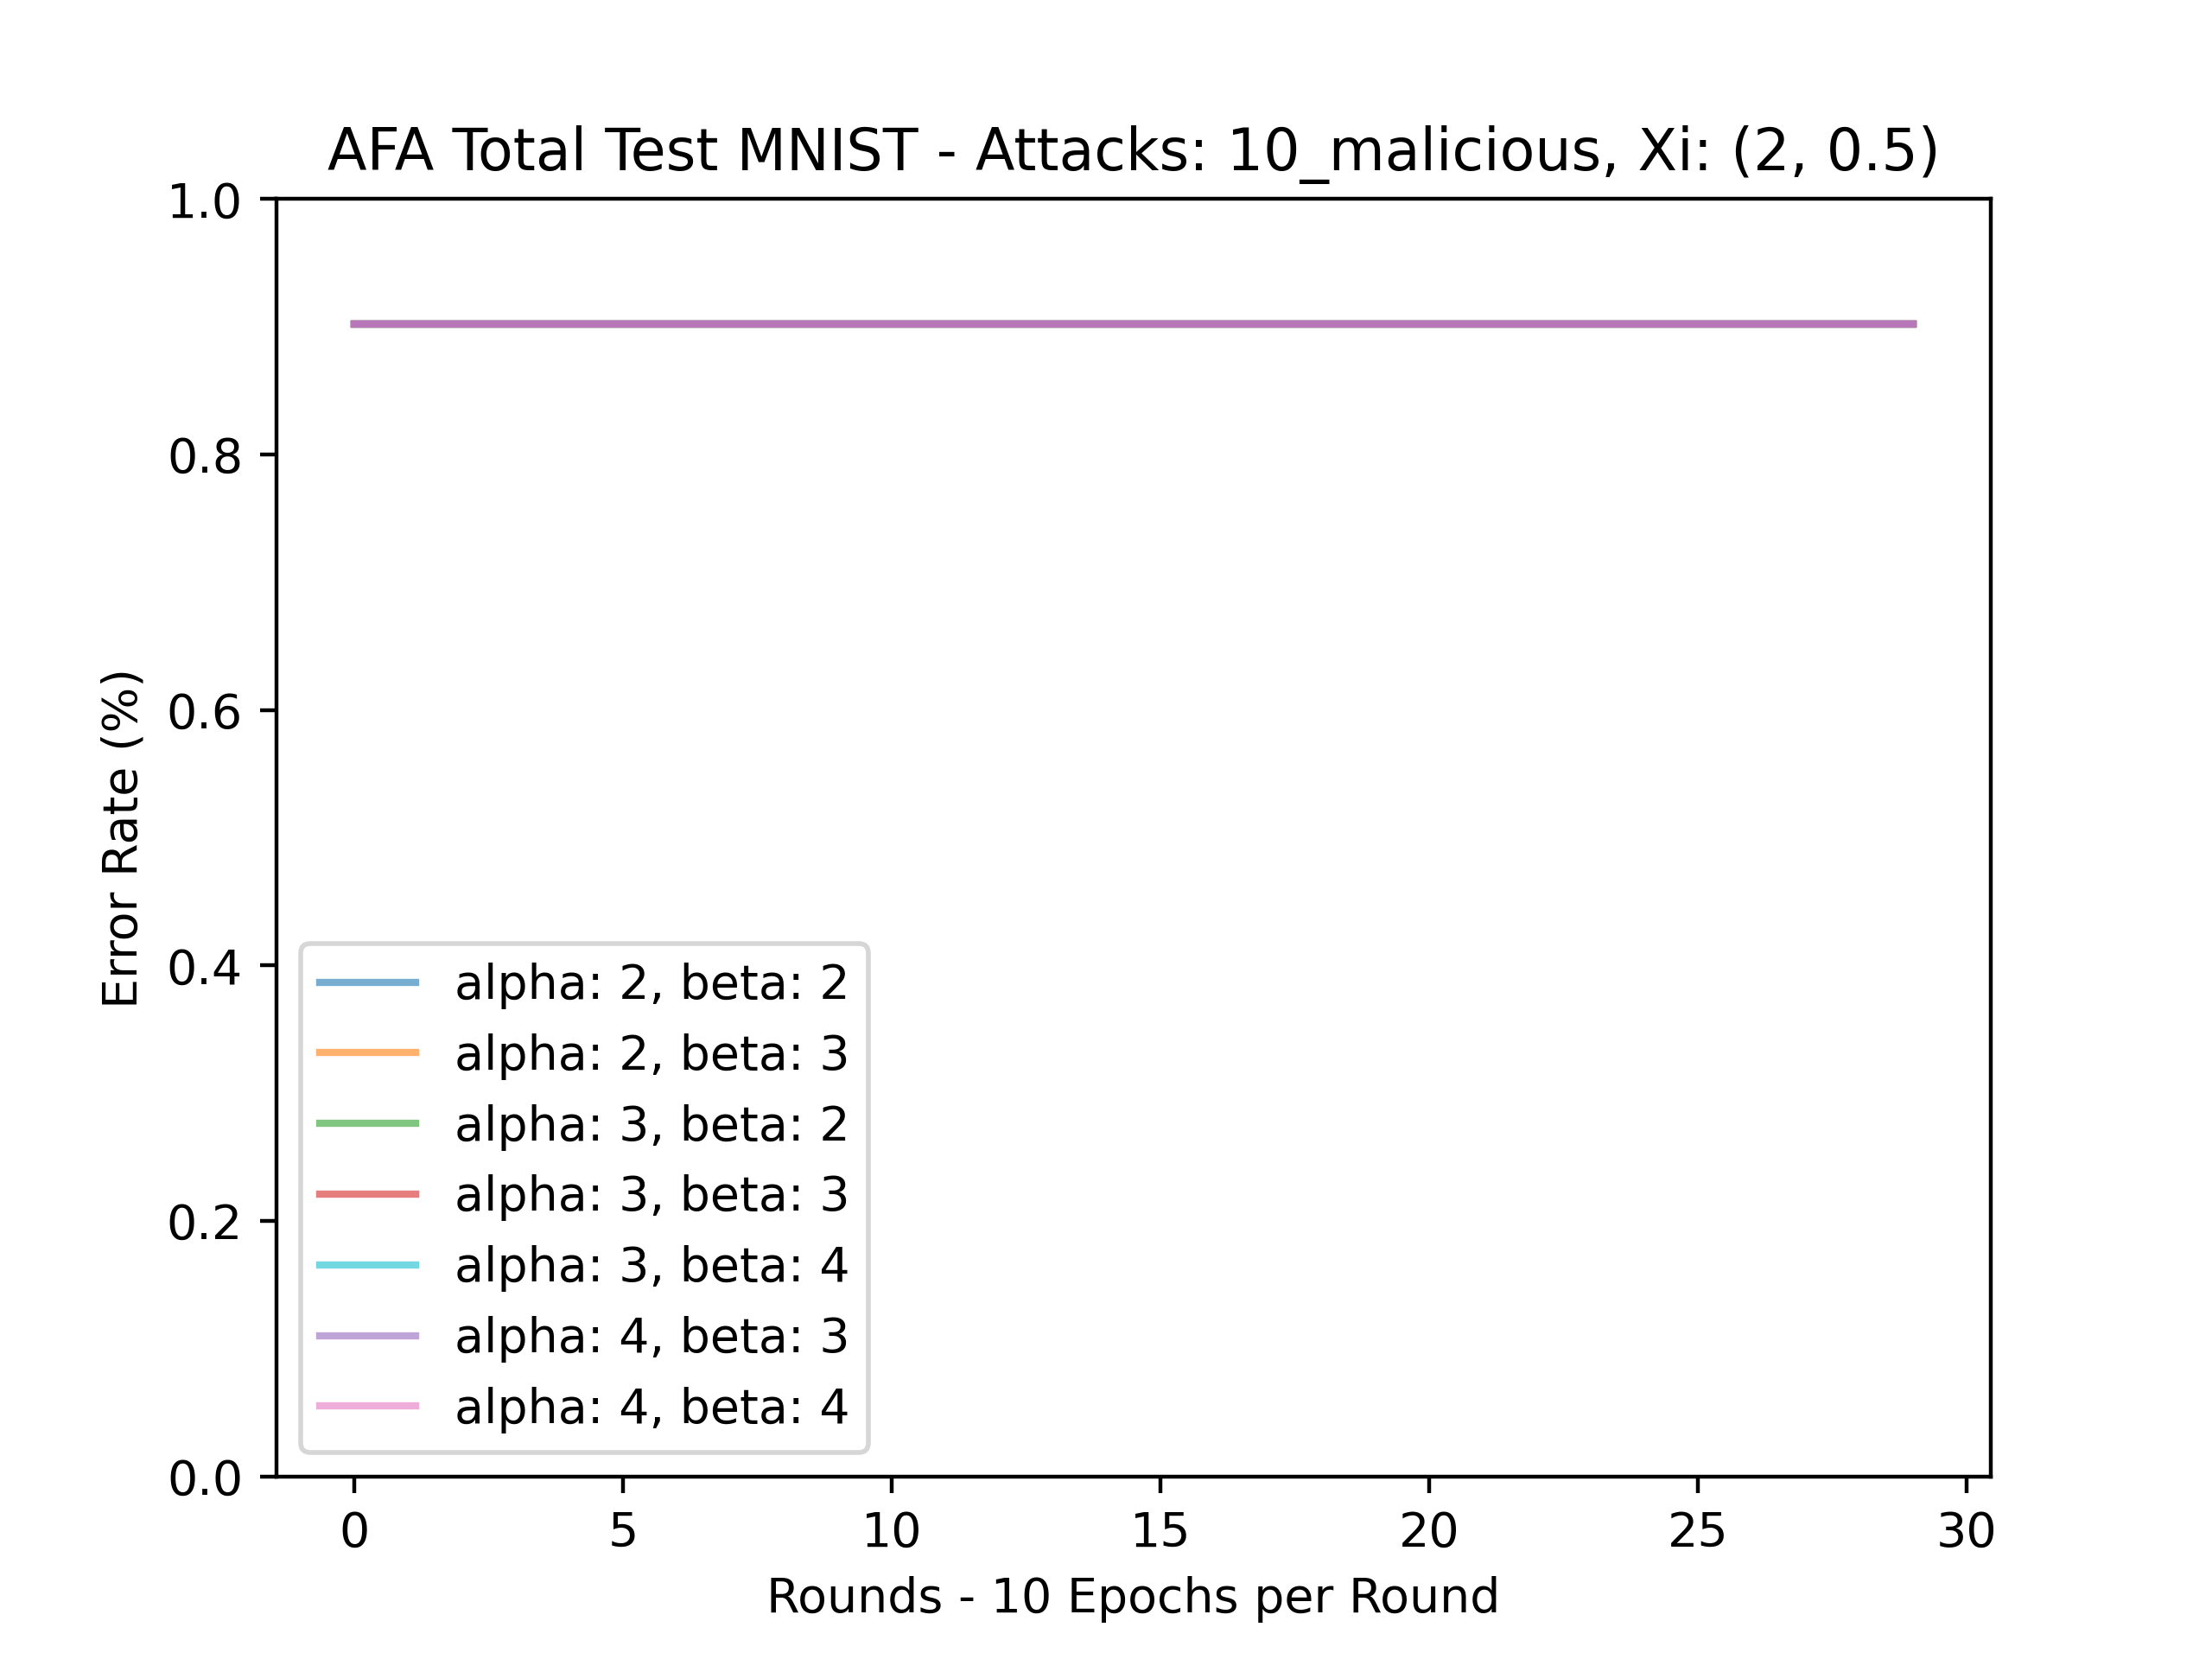
\includegraphics[scale=0.5]{initial/graphs/malicious_afa.png}
	\caption{10 Malicious clients in AFA}
	\label{fig:mal_afa}
\end{figure}

\begin{figure}[htbp]
	\centering
    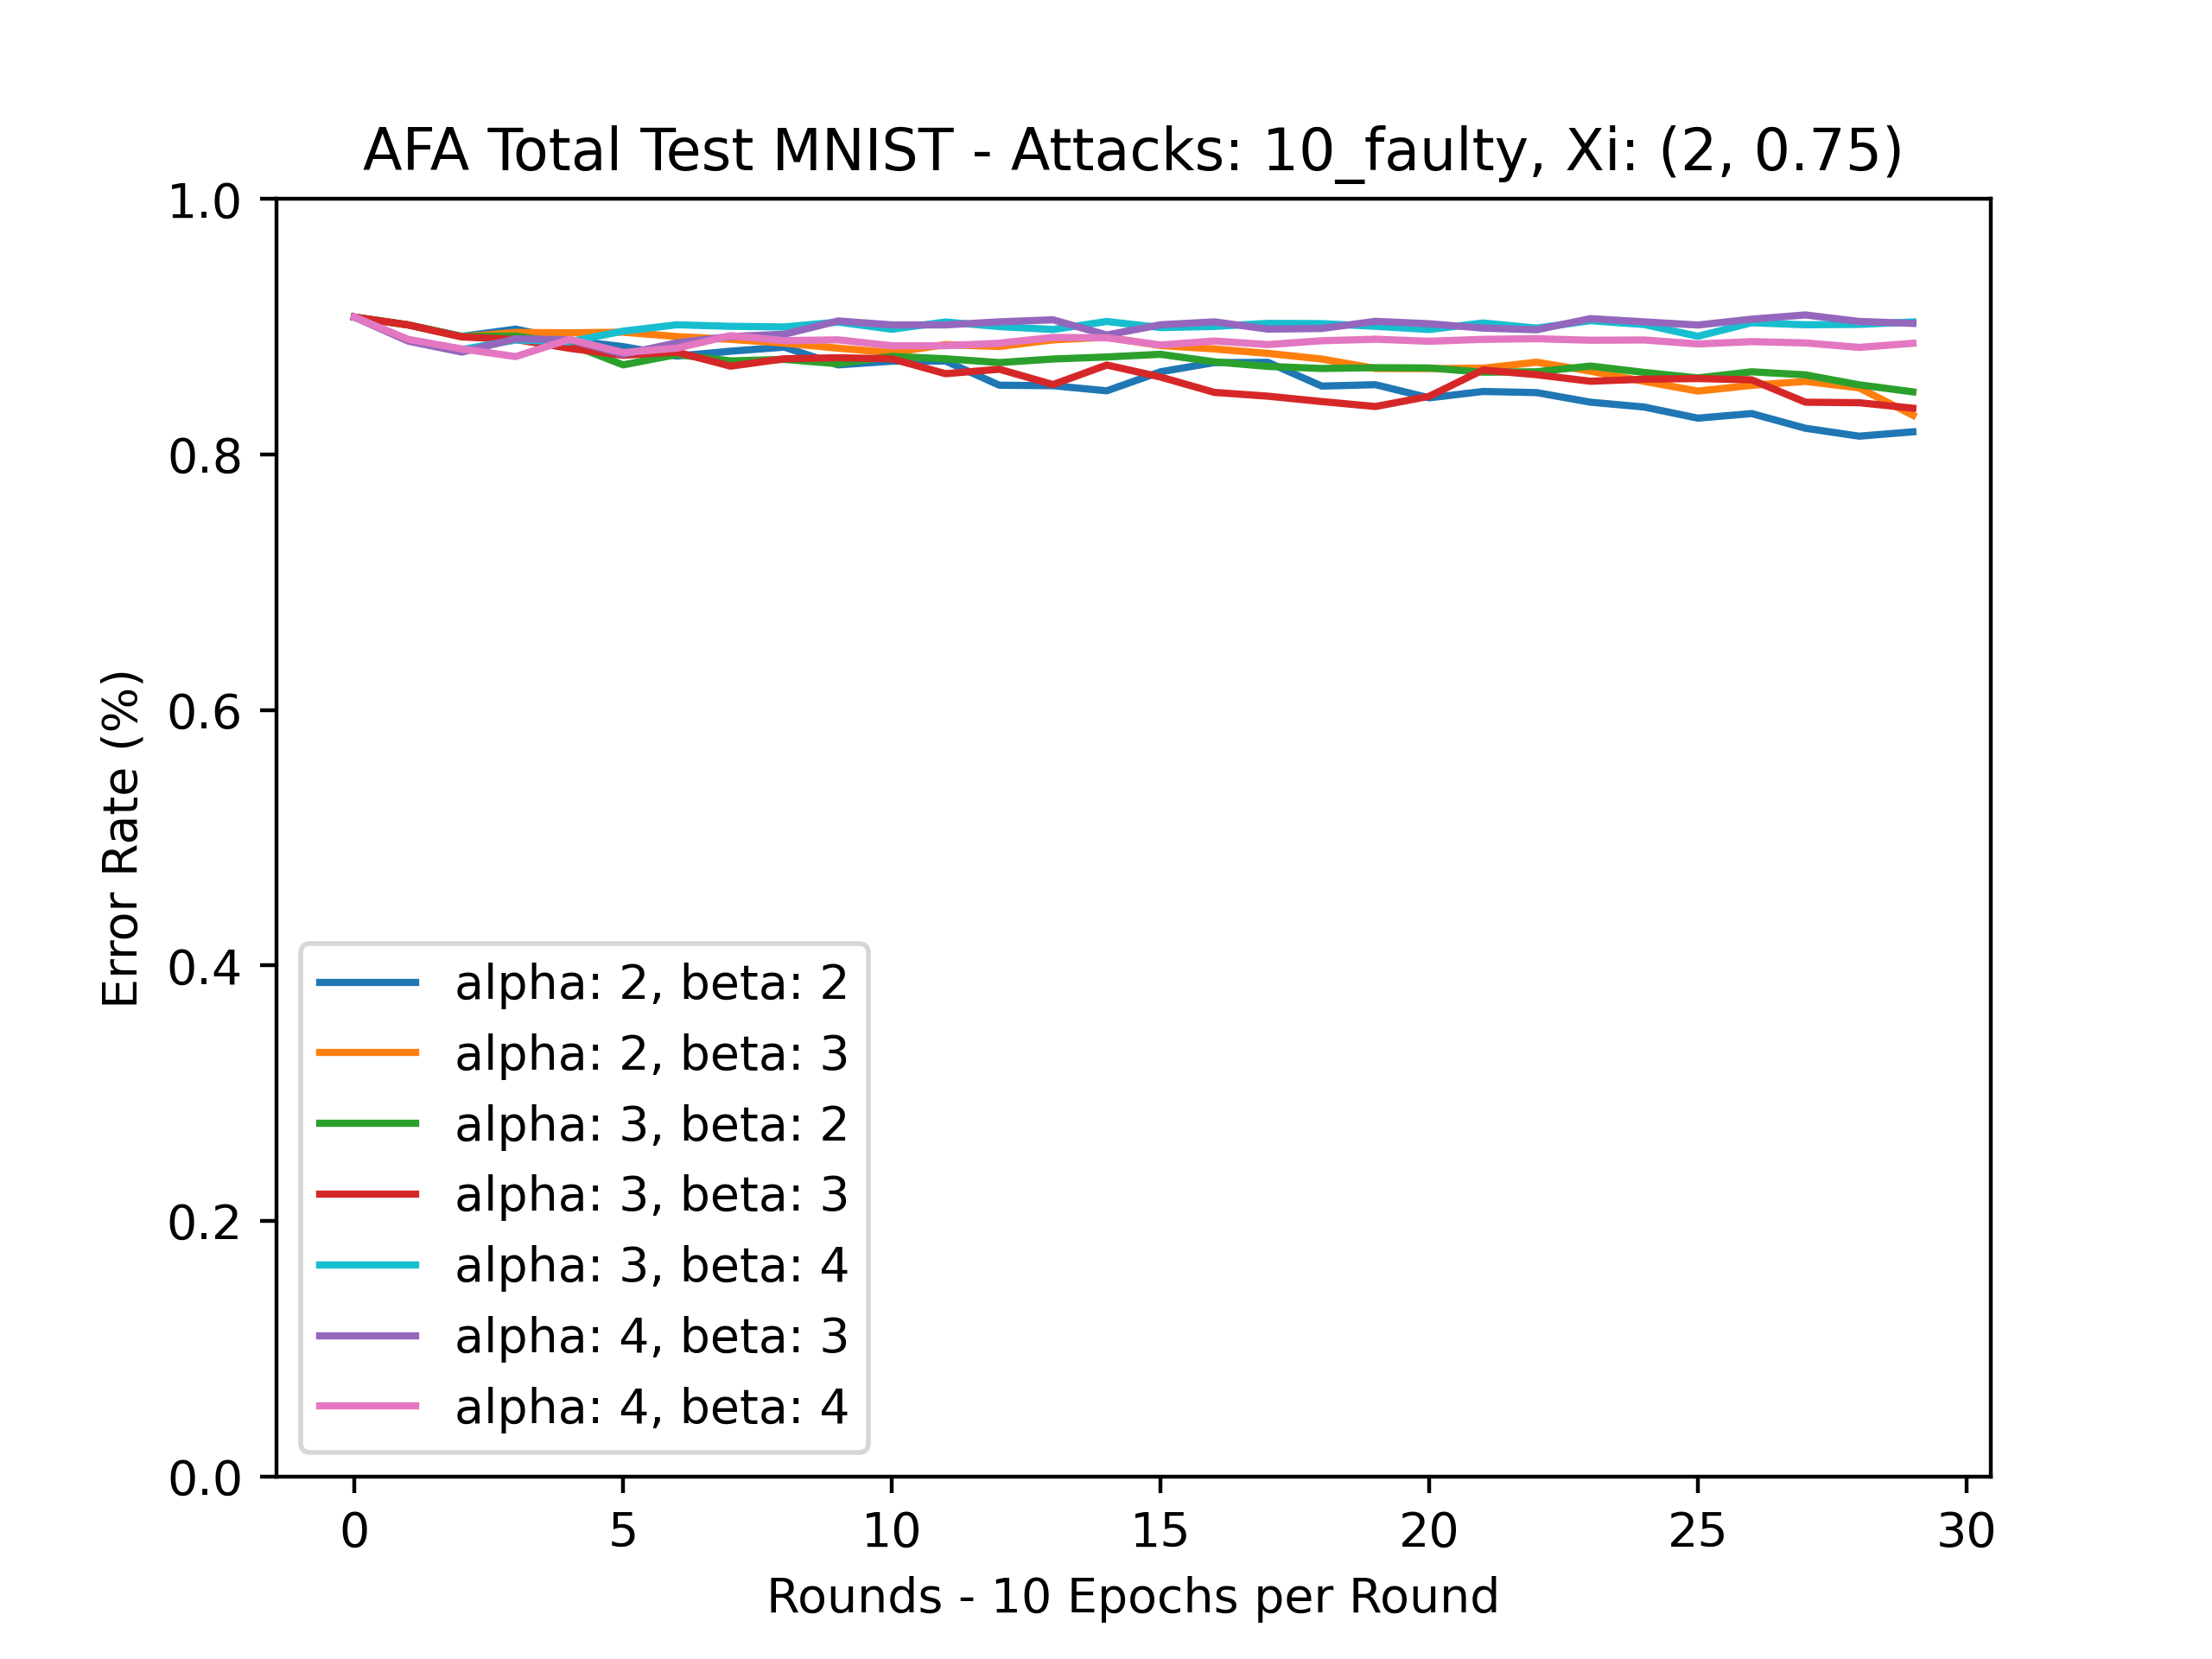
\includegraphics[scale=0.5]{initial/graphs/afa_2_0.75.png}
	\caption{AFA - Xi: 2, DeltaXi: 0.75}
	\label{fig:afa_2_0.75}
\end{figure}

\begin{figure}[htbp]
	\centering
    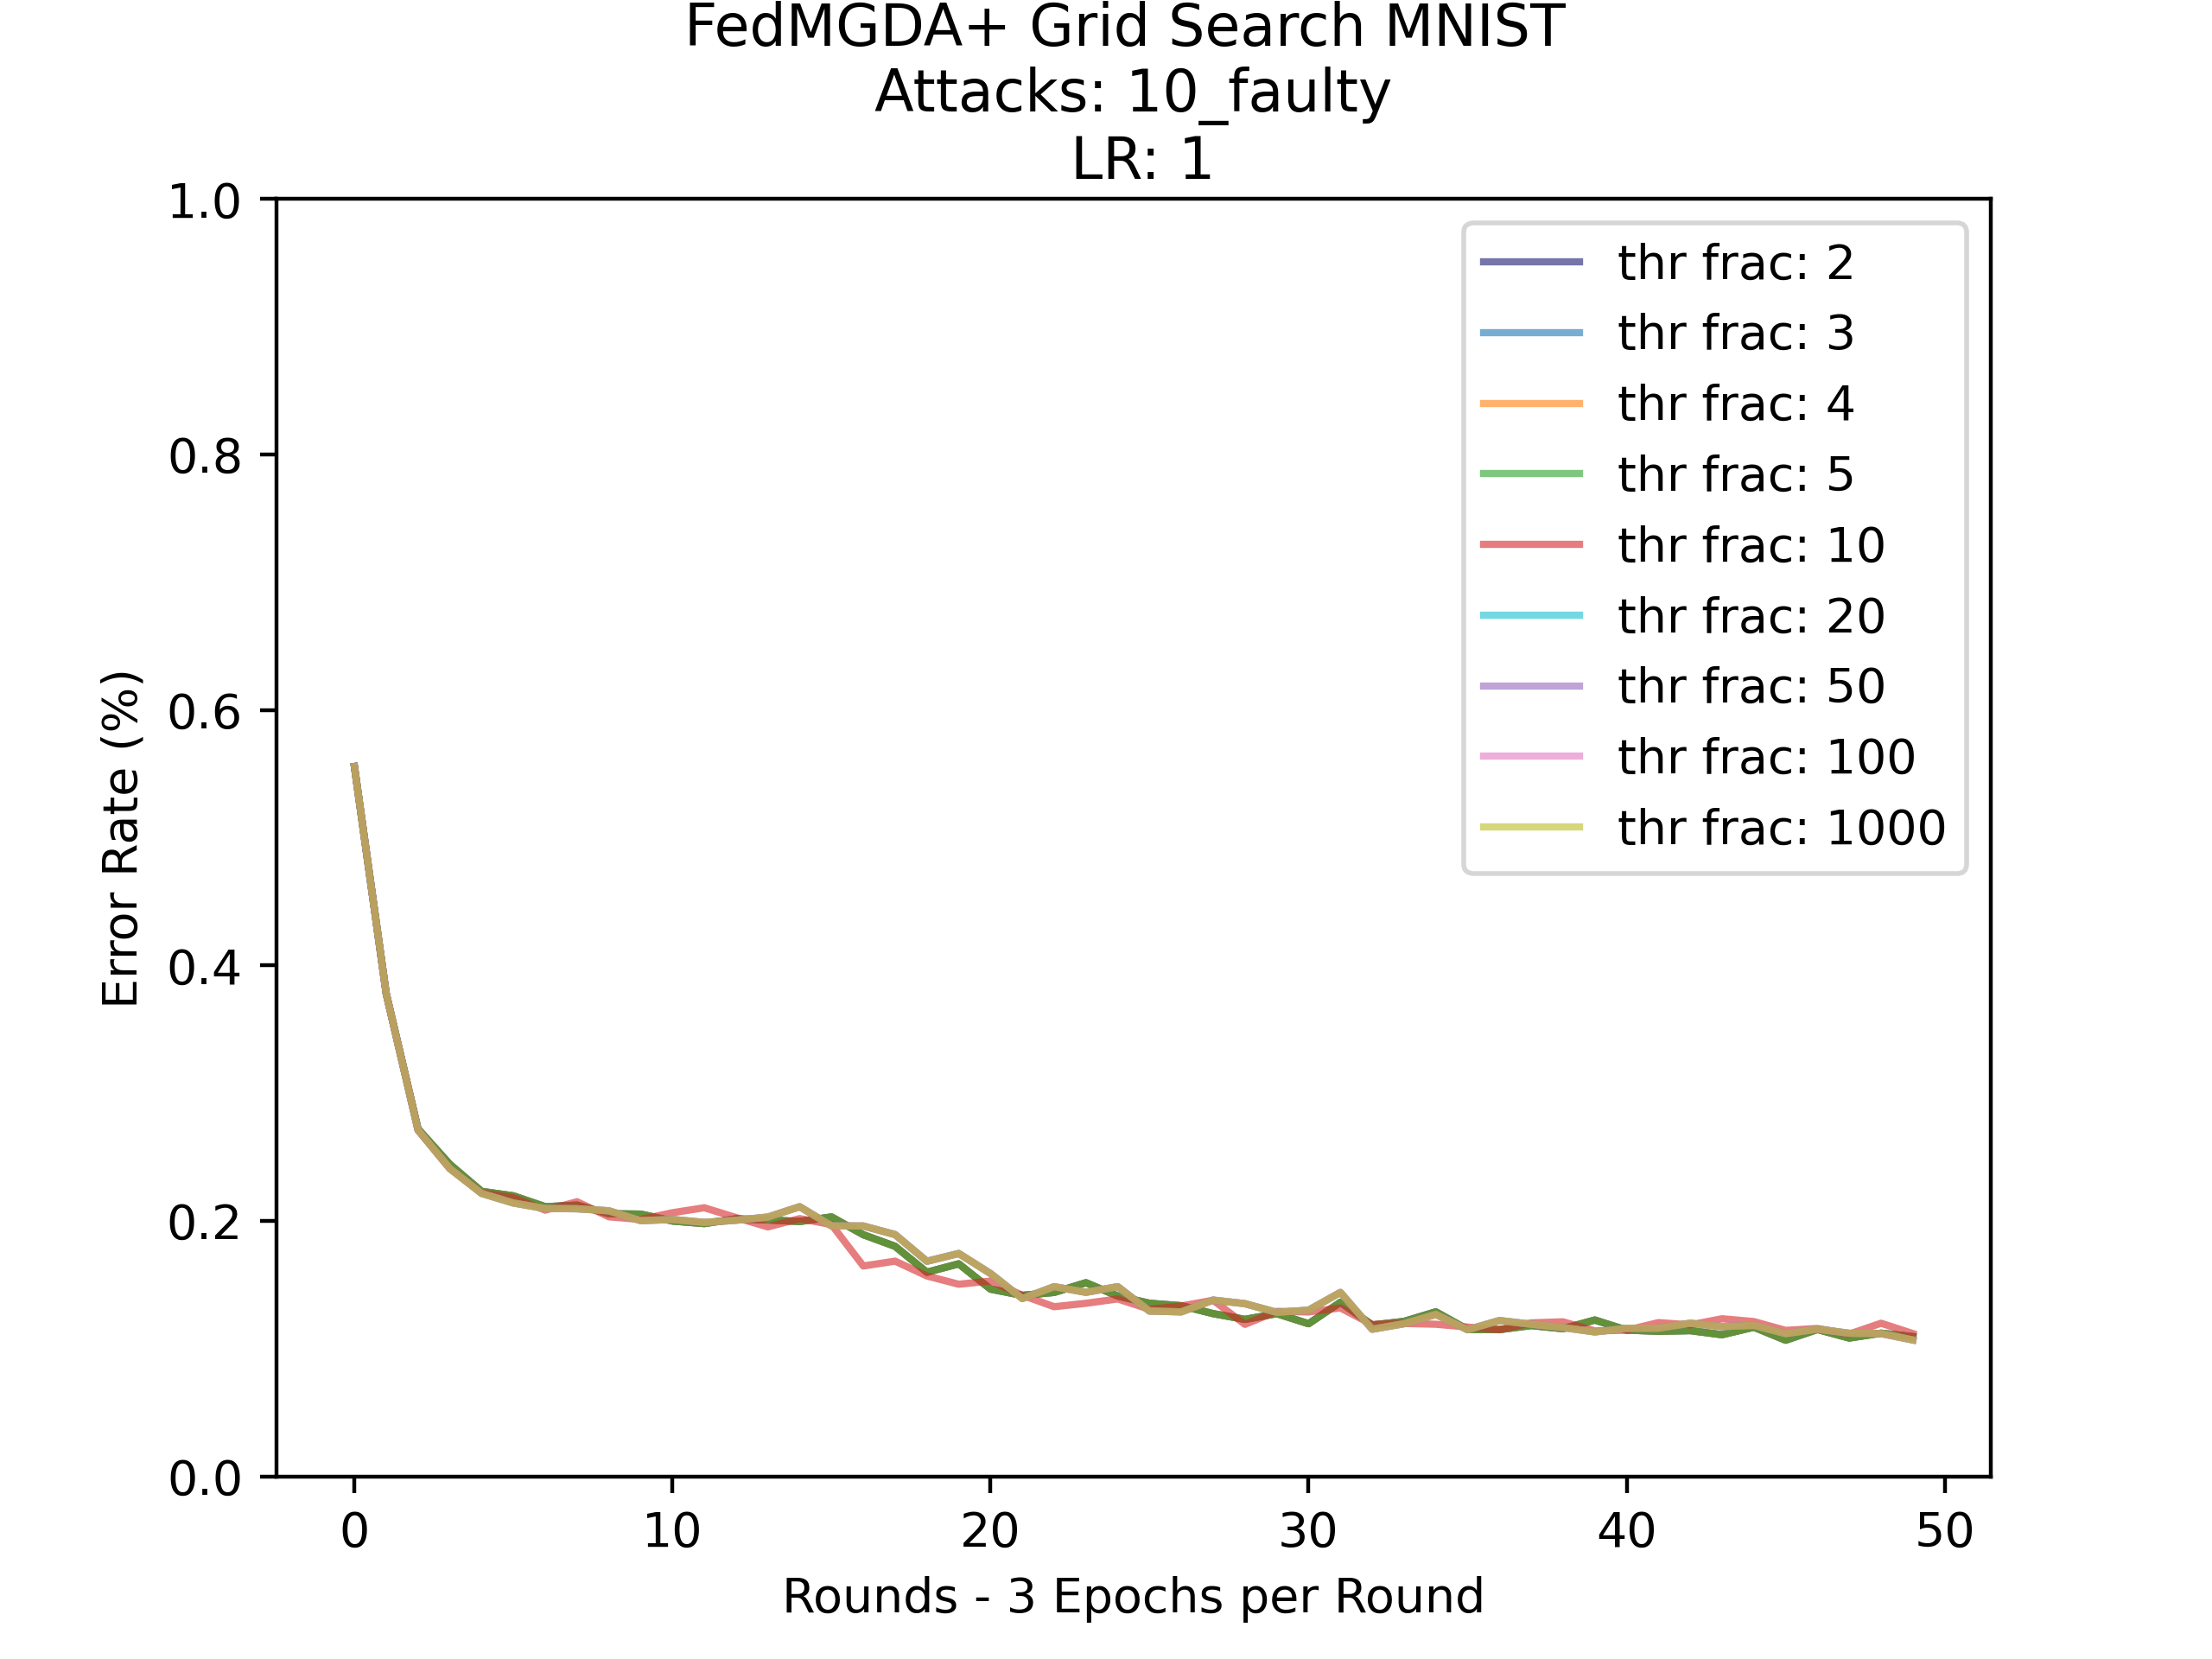
\includegraphics[scale=0.5]{initial/graphs/mgda_var.png}
	\caption{FedMGDA+ Threshold Variance Demo}
	\label{fig:mgda_var}
\end{figure}

\begin{figure}[htbp]
	\centering
    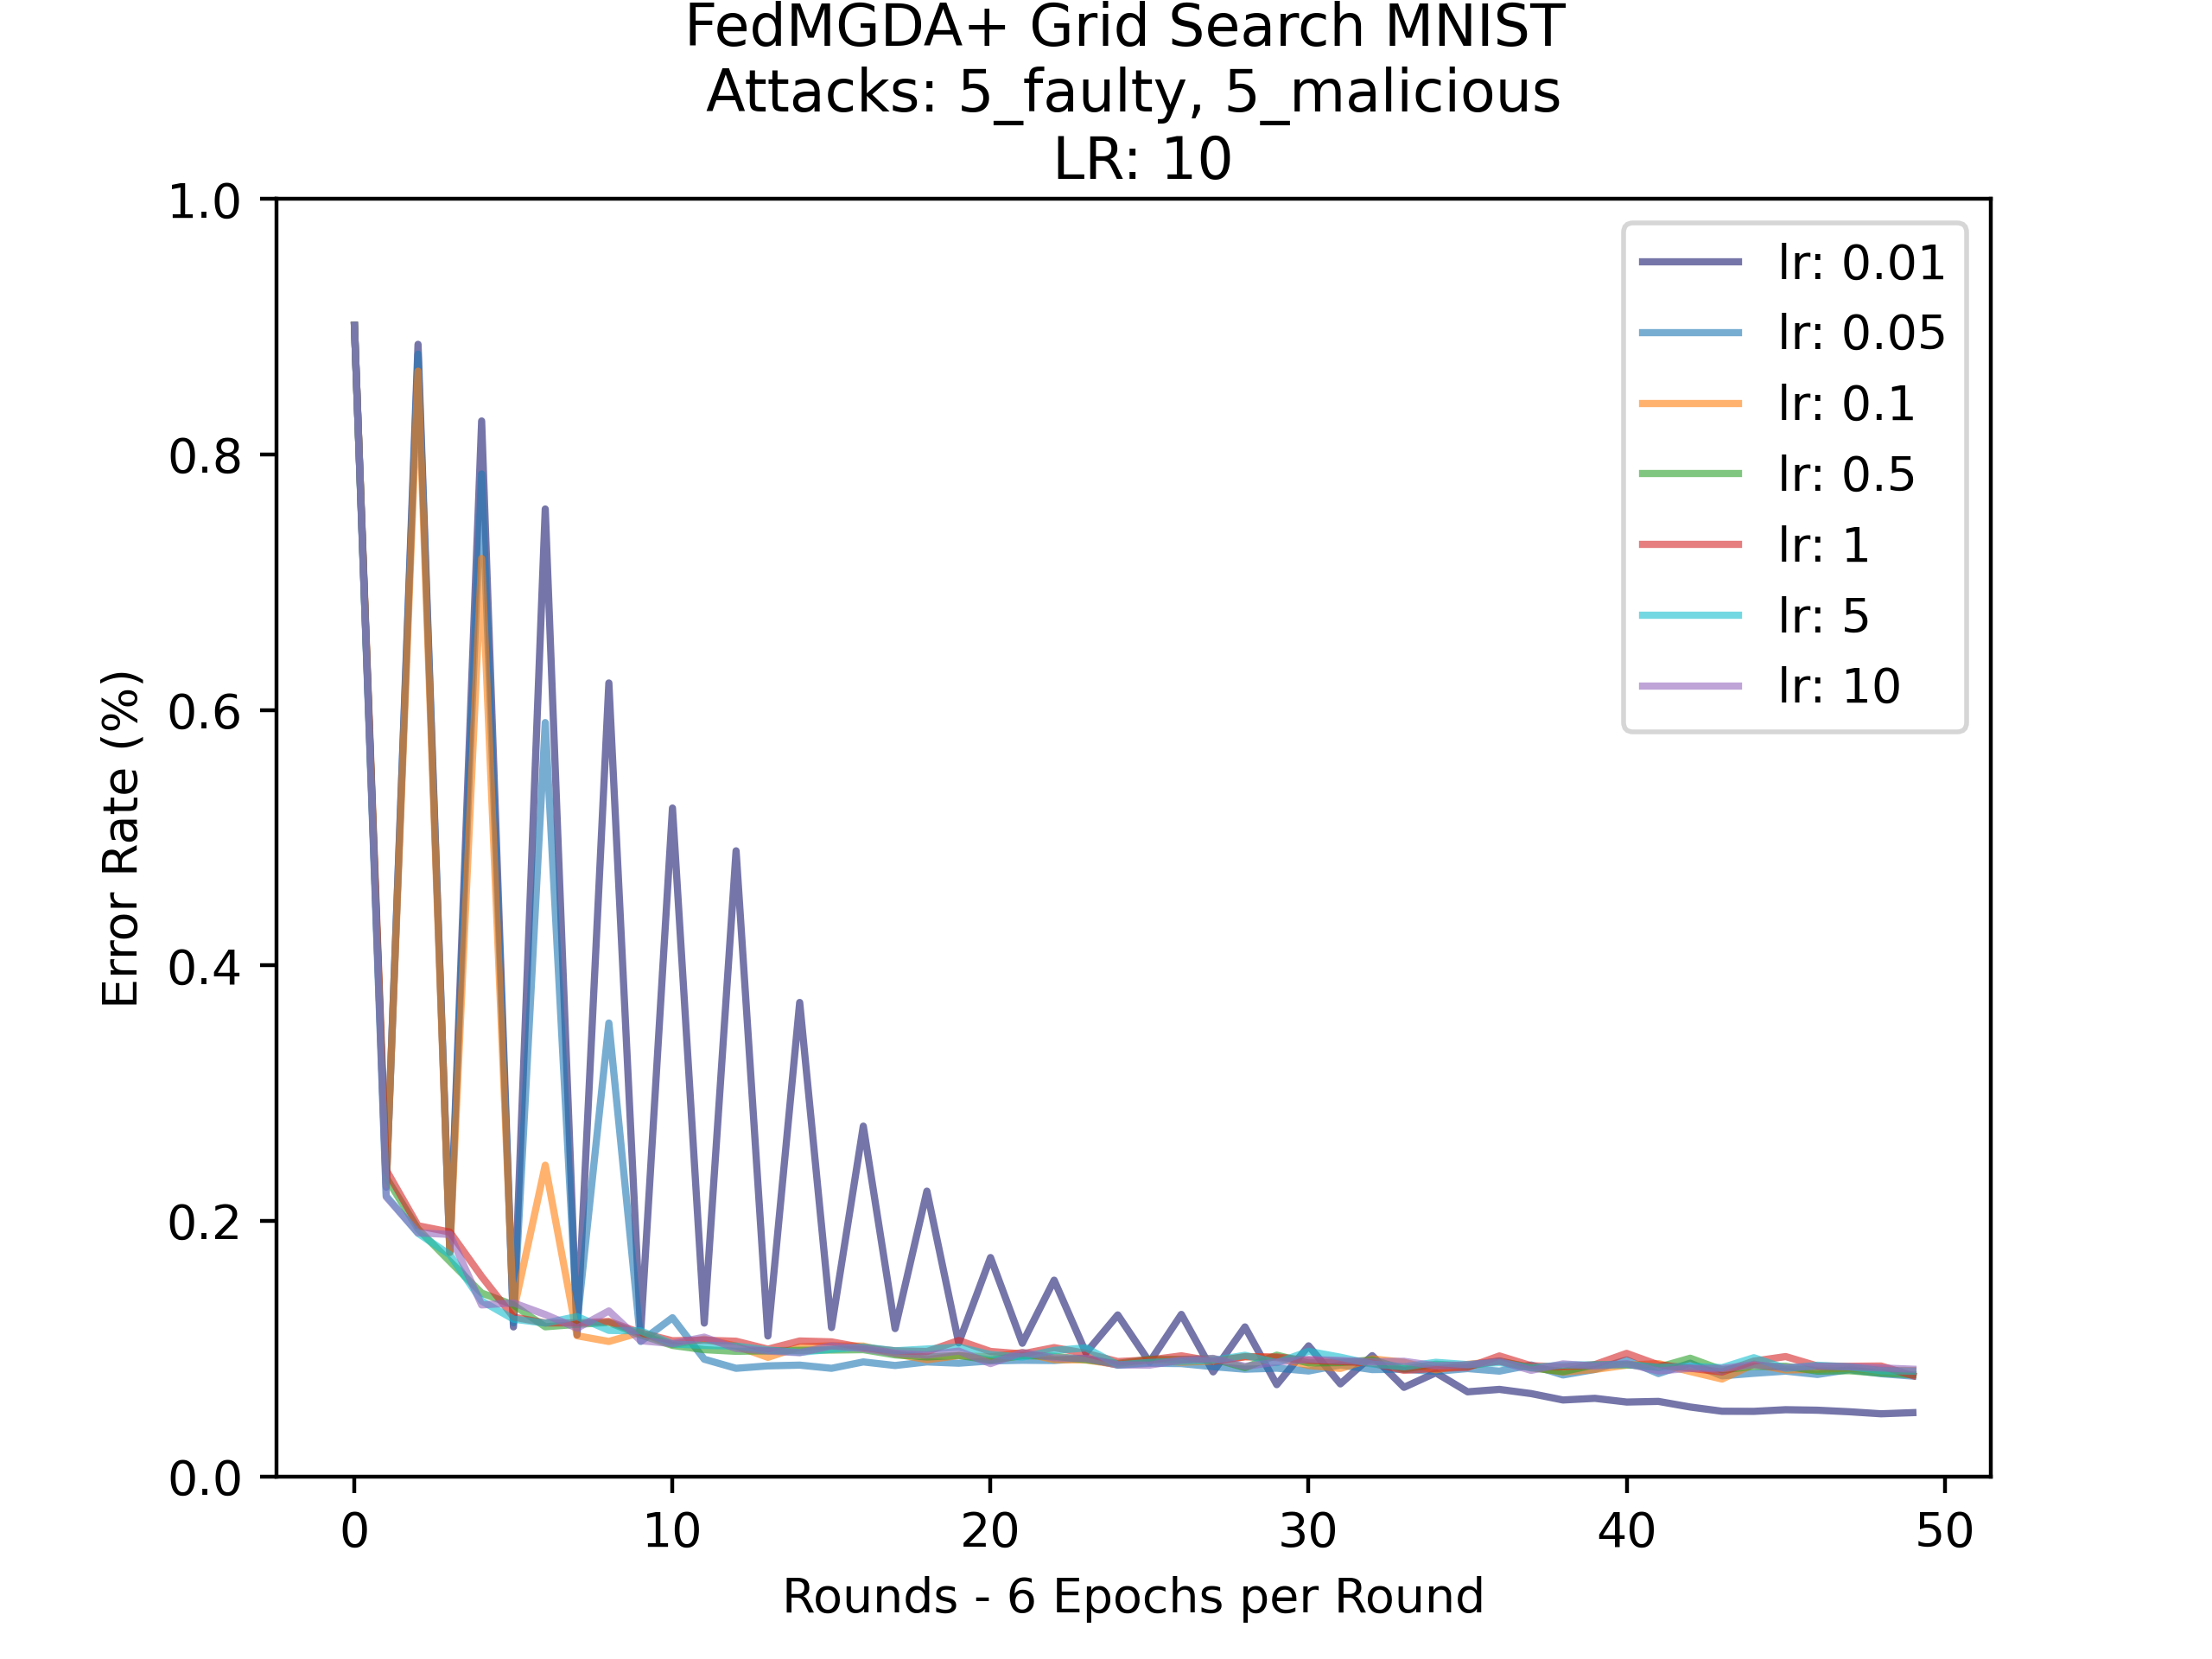
\includegraphics[scale=0.5]{initial/graphs/fake_good.png}
	\caption{FedMGDA+ Quick Convergence}
	\label{fig:fake_good}
\end{figure}

\begin{figure}[htbp]
	\centering
    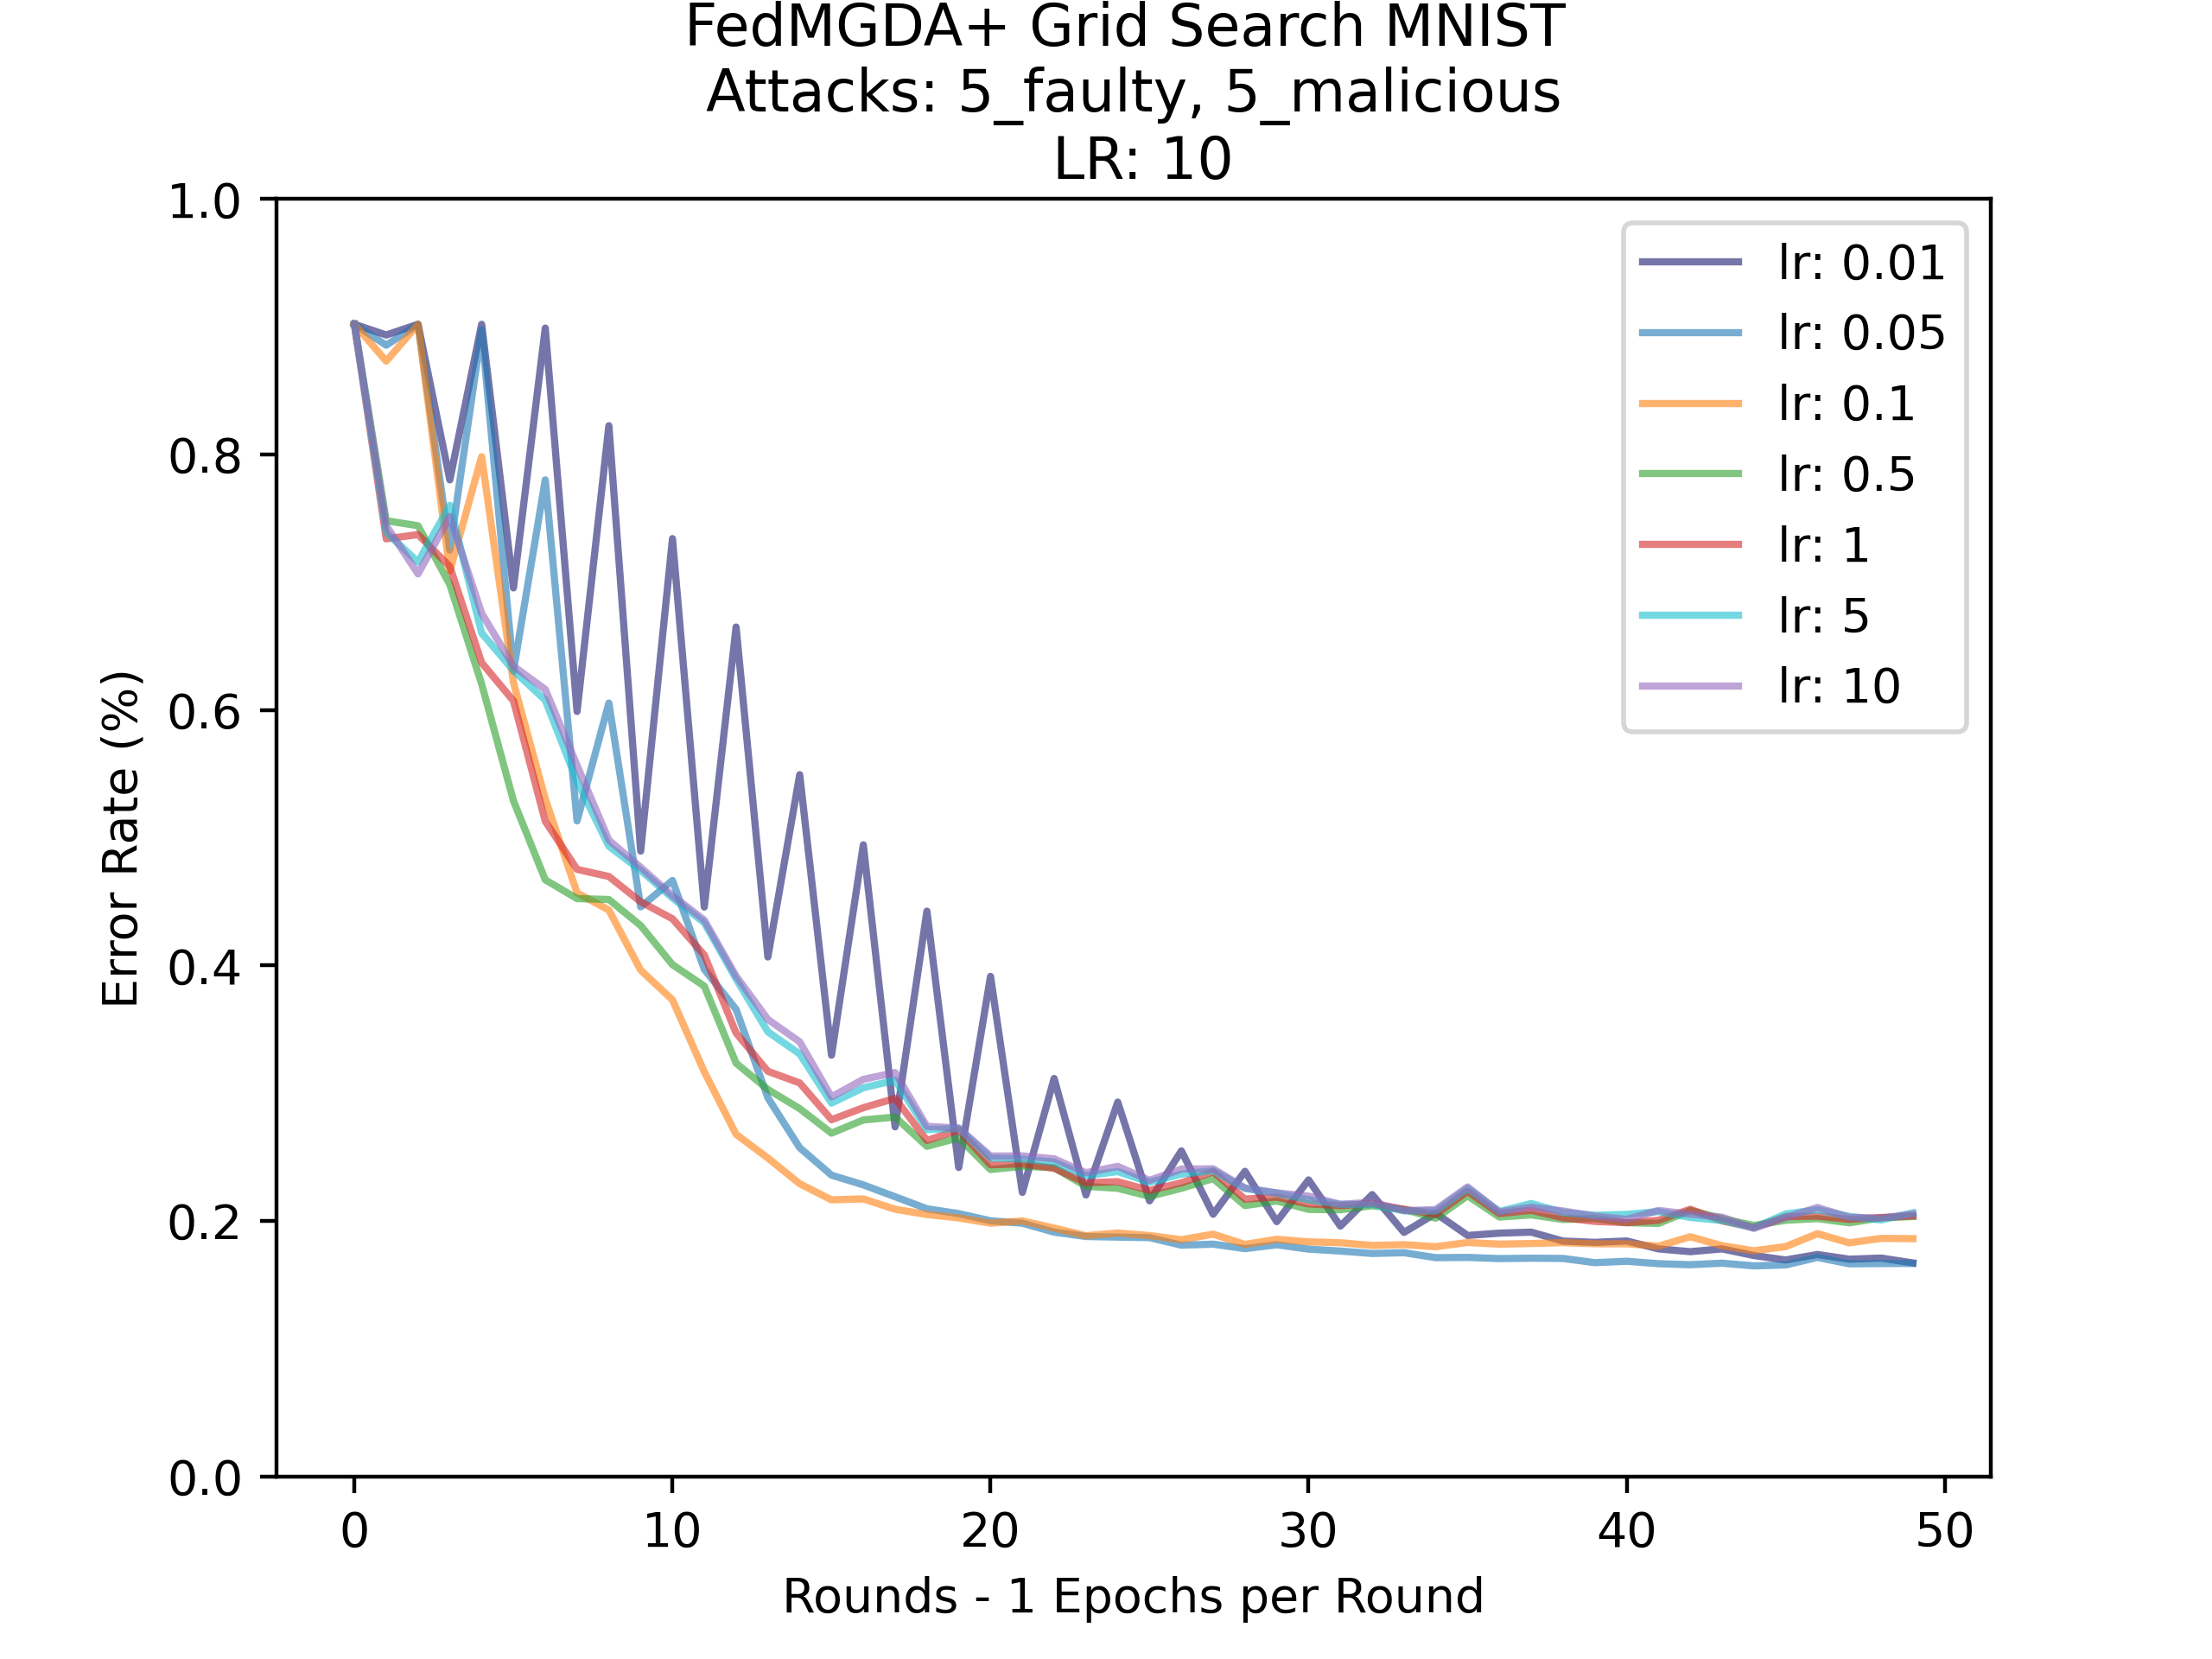
\includegraphics[scale=0.5]{initial/graphs/1epoch_grid.png}
	\caption{FedMGDA+ with No Benign Blocked but High Error Rate}
	\label{fig:1epoch_grid}
\end{figure}

\begin{figure}[htbp]
	\centering
    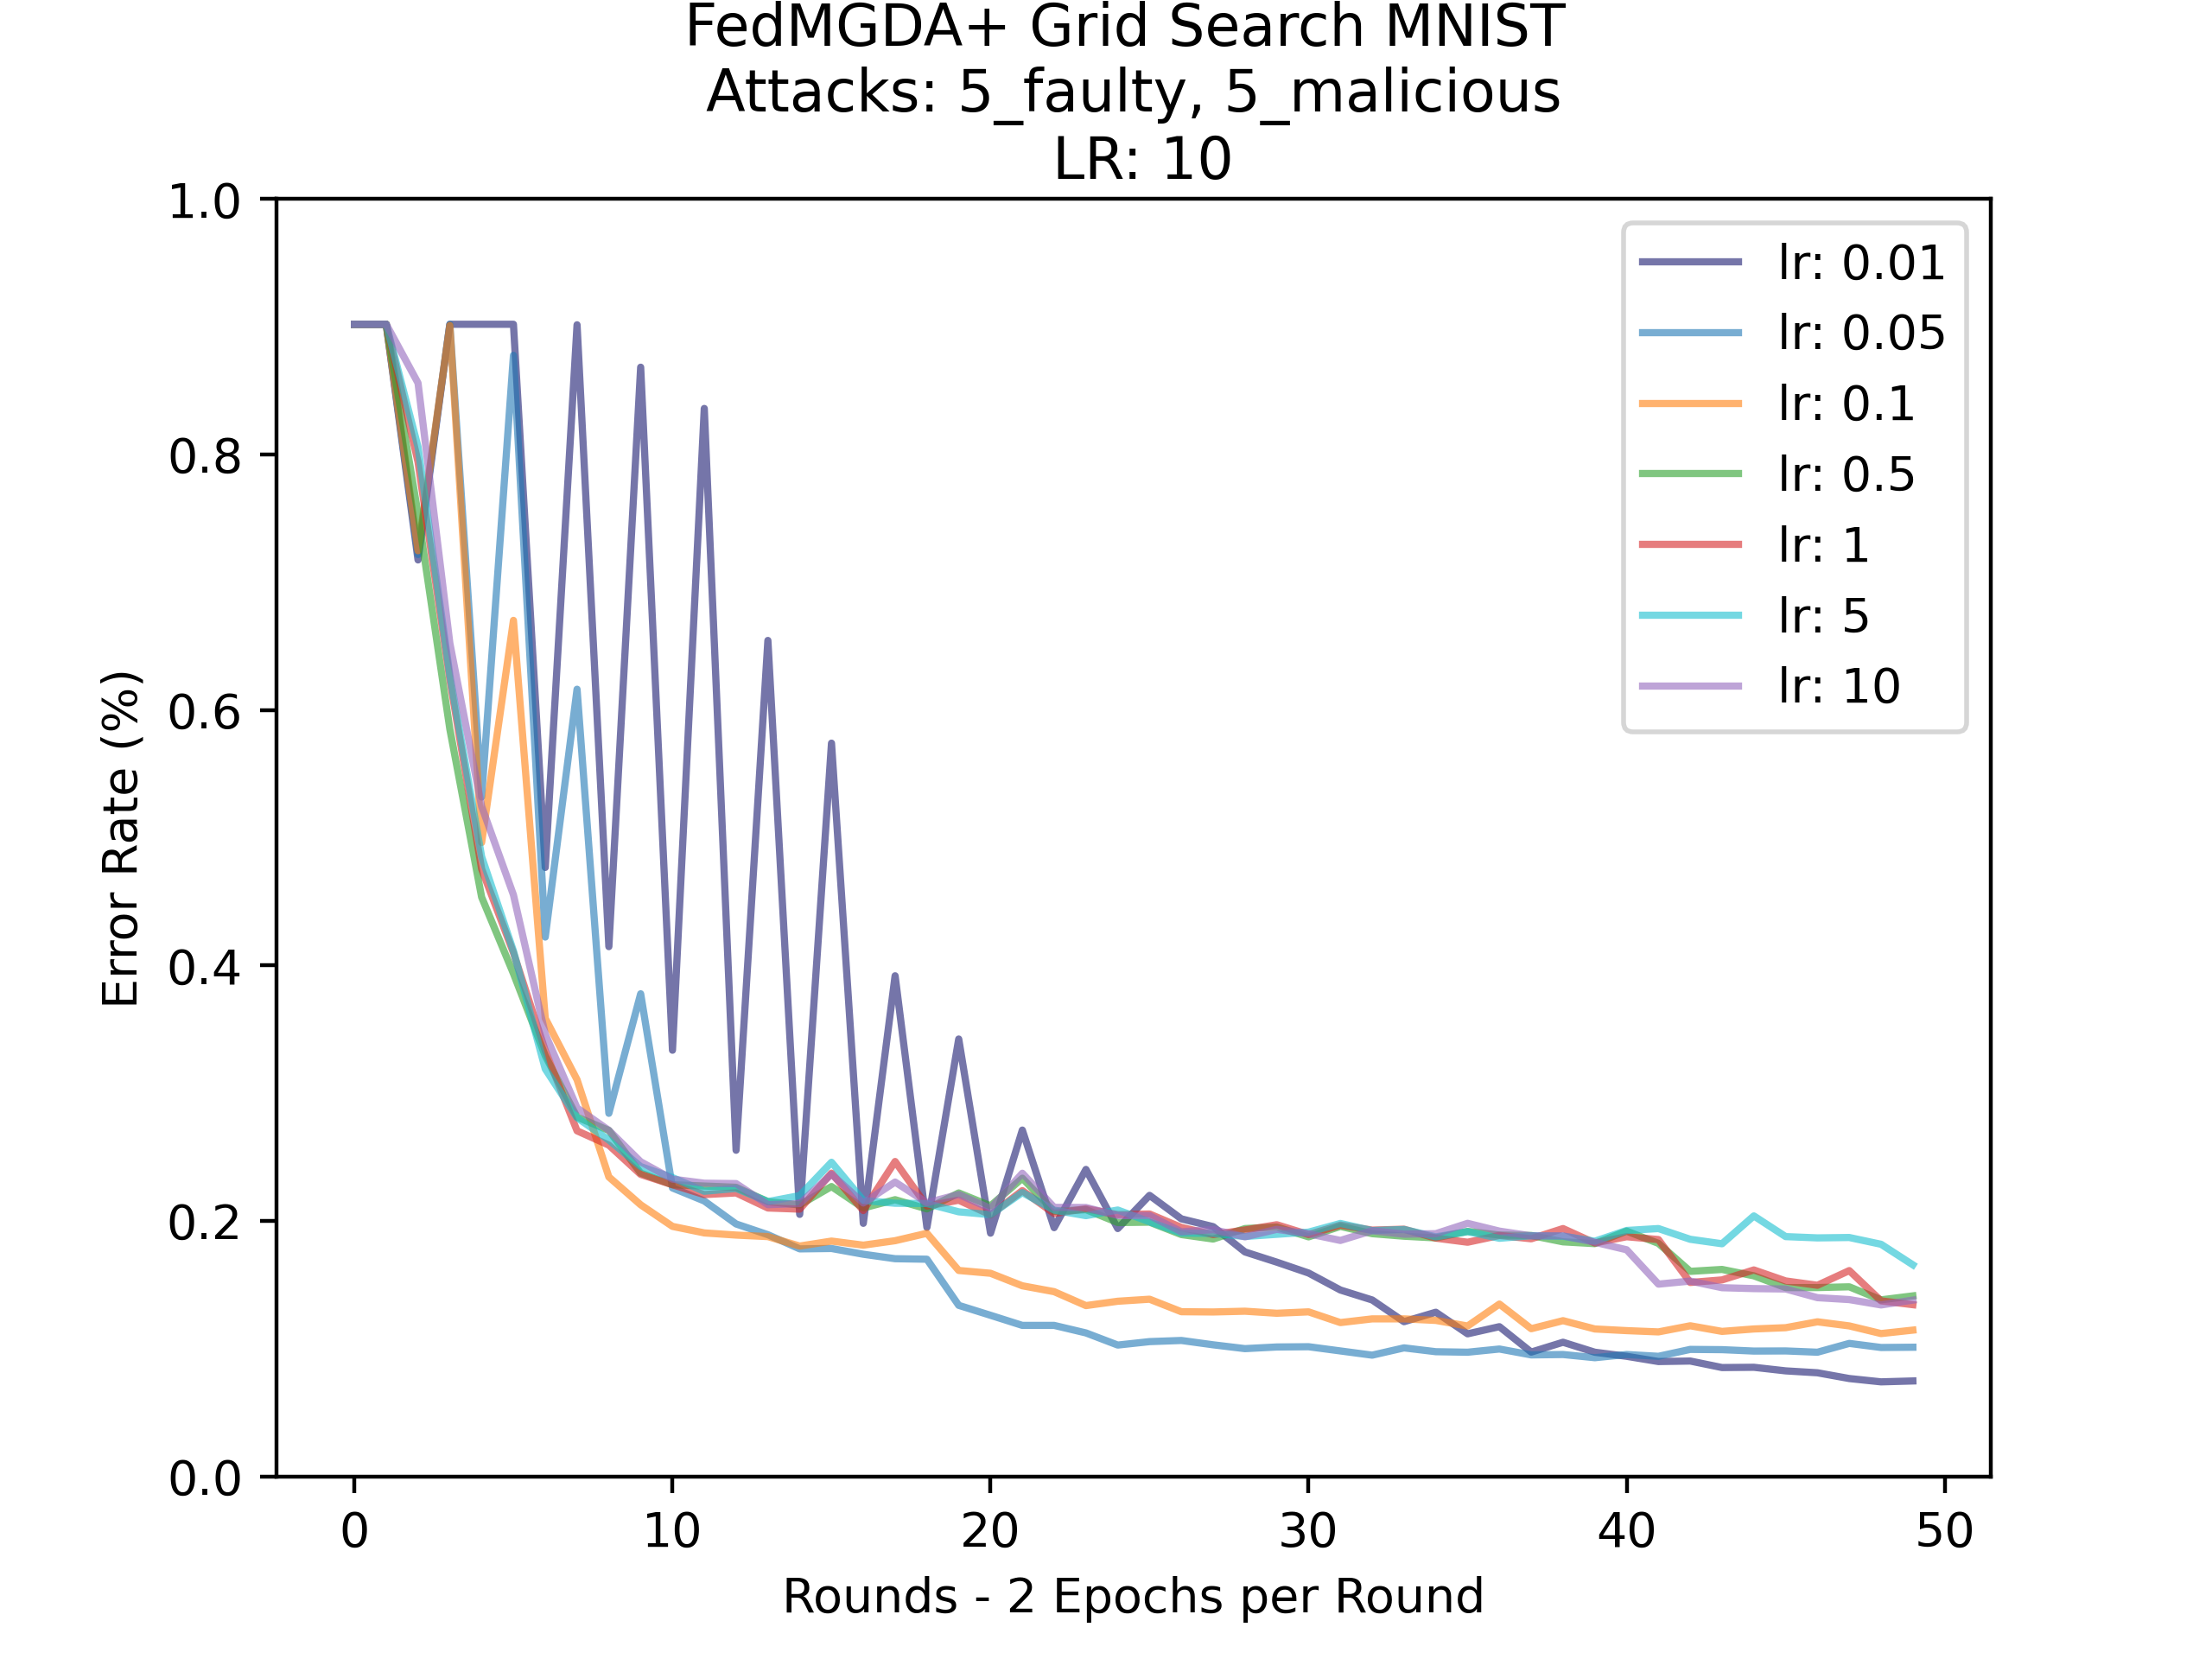
\includegraphics[scale=0.5]{initial/graphs/2epoch_grid.png}
	\caption{FedMGDA+ Benign Blocked Late but Low Error Rate}
	\label{fig:2epoch_grid}
\end{figure}

\begin{figure}[htbp]
	\centering
    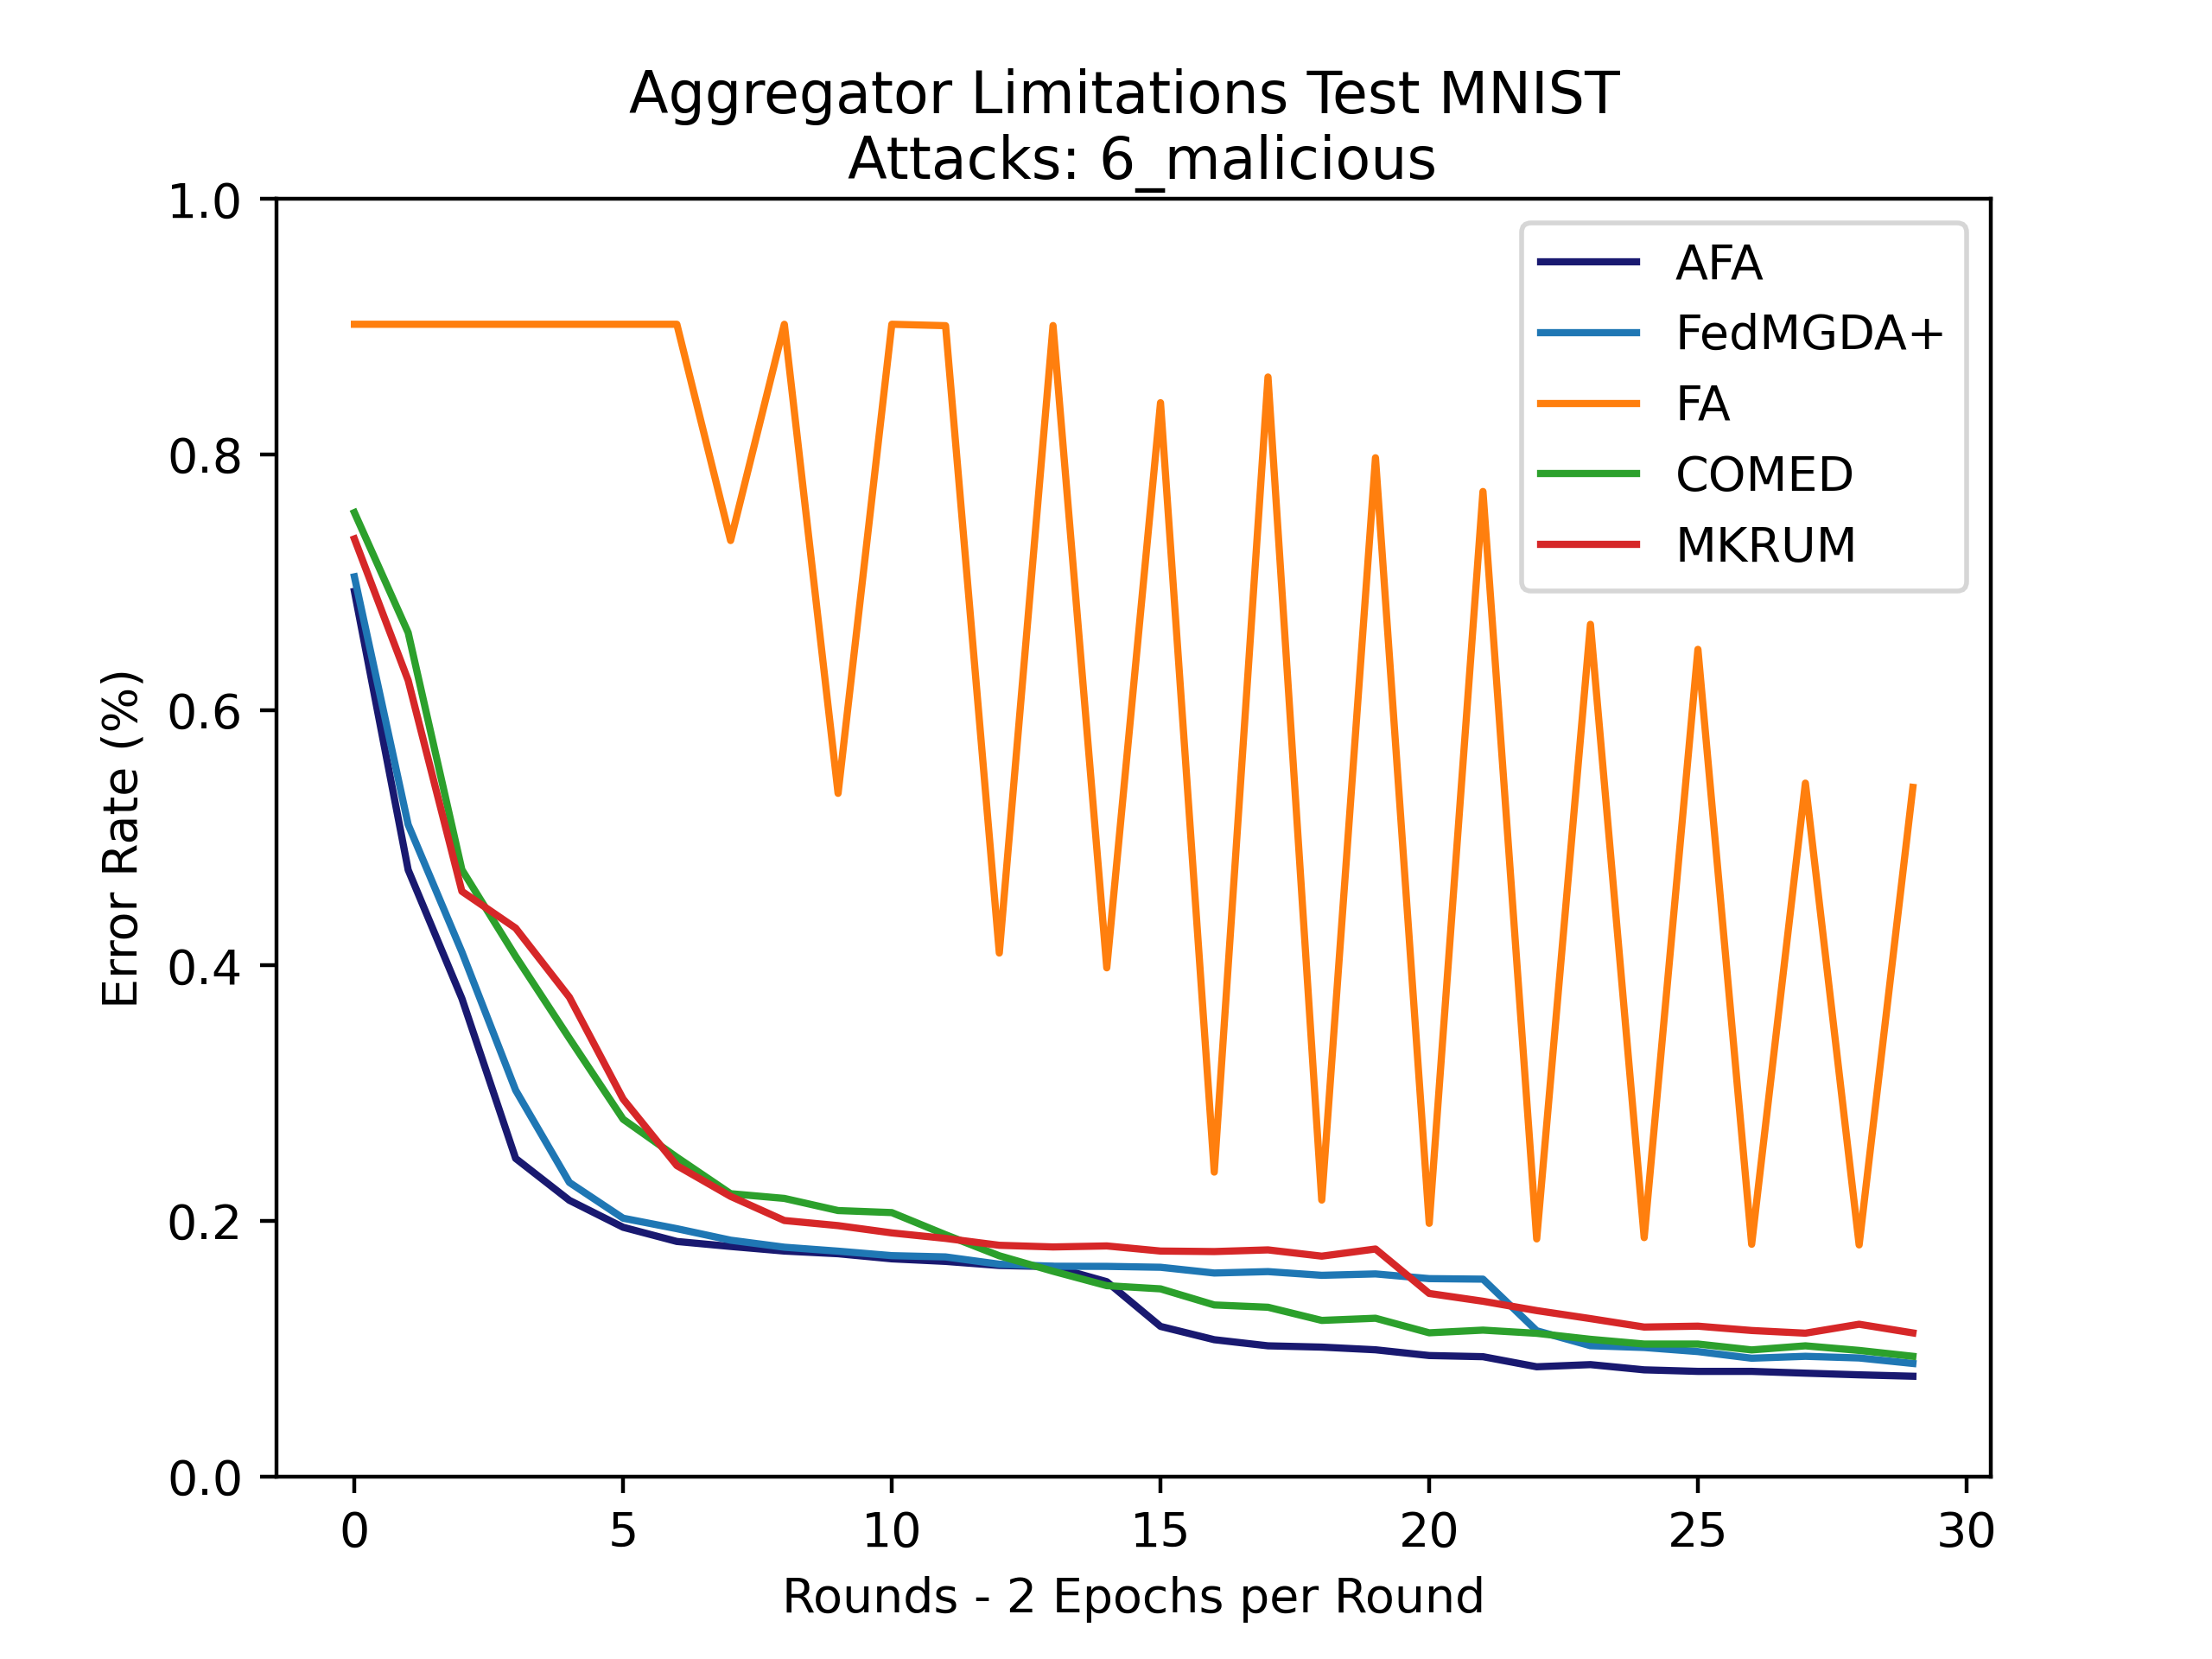
\includegraphics[scale=0.5]{initial/graphs/6_malicious.png}
	\caption{FedAvg Failing to Converge with Noticeable Damage in the Training Process}
	\label{fig:6mal}
\end{figure}

\begin{figure}[htbp]
	\centering
    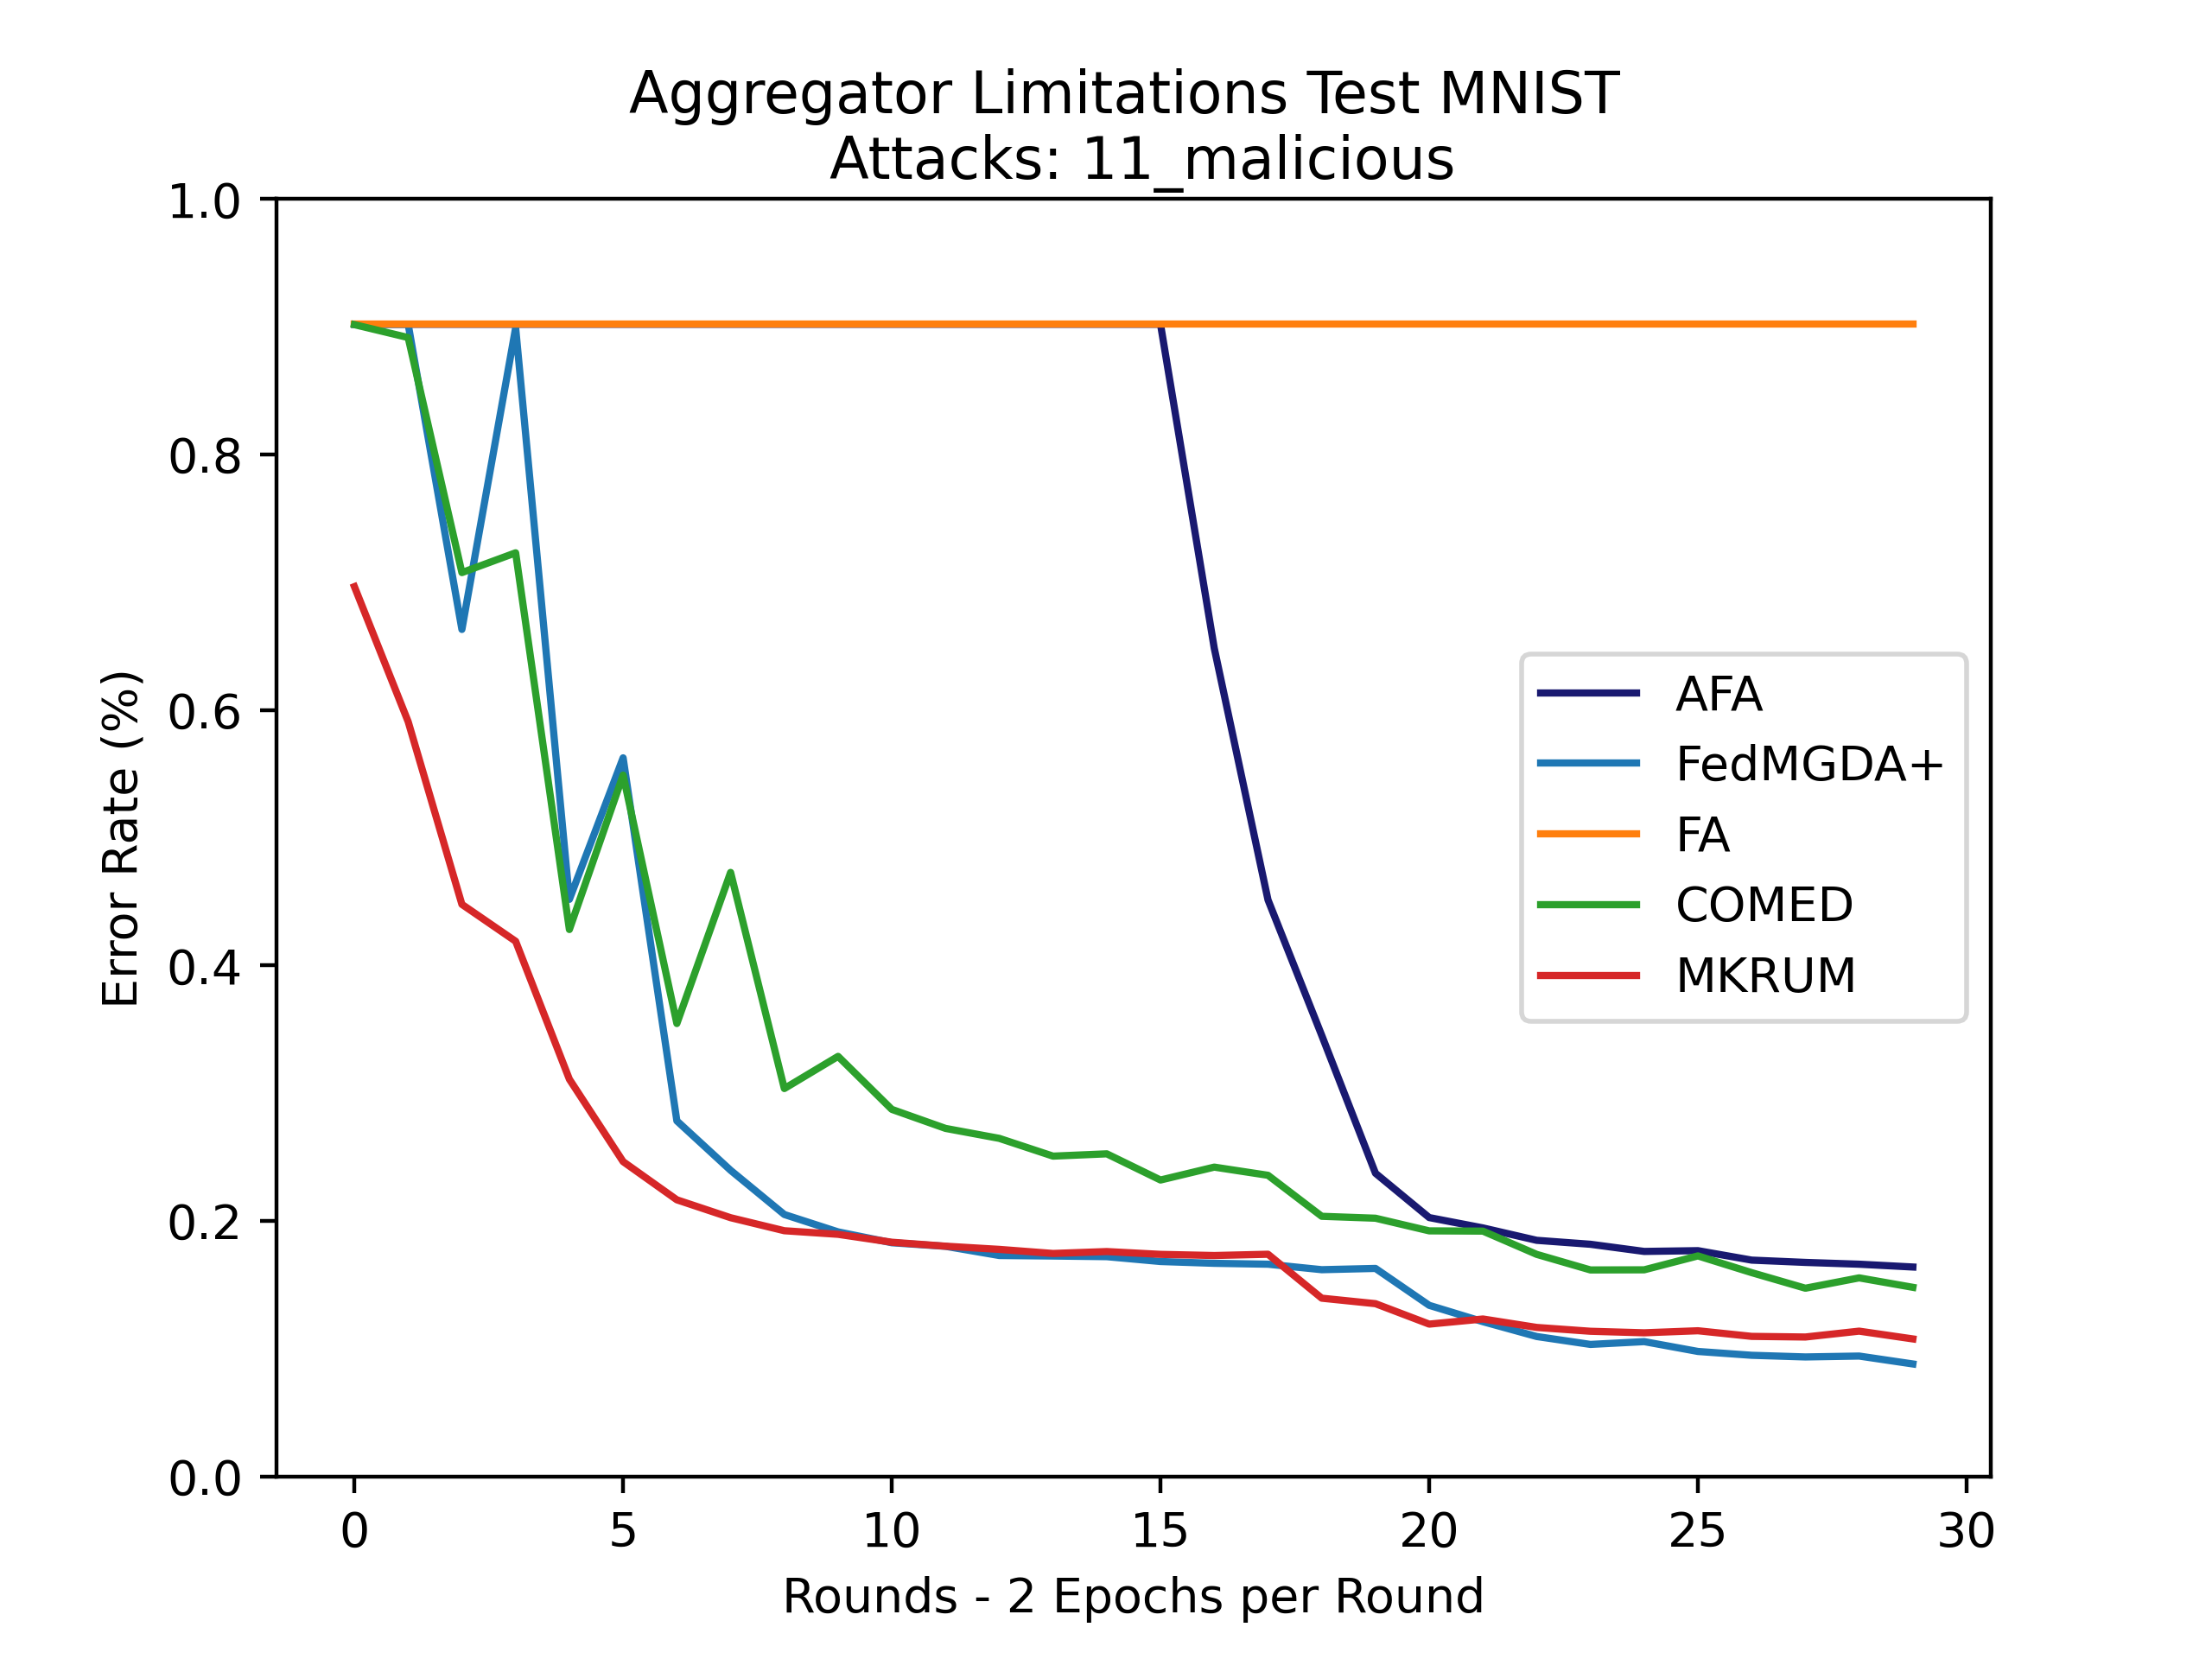
\includegraphics[scale=0.5]{initial/graphs/11_malicious.png}
	\caption{The Beginning of the End for Robust Aggregators with Malicious Clients}
	\label{fig:11mal}
\end{figure}

\begin{figure}[htbp]
	\centering
    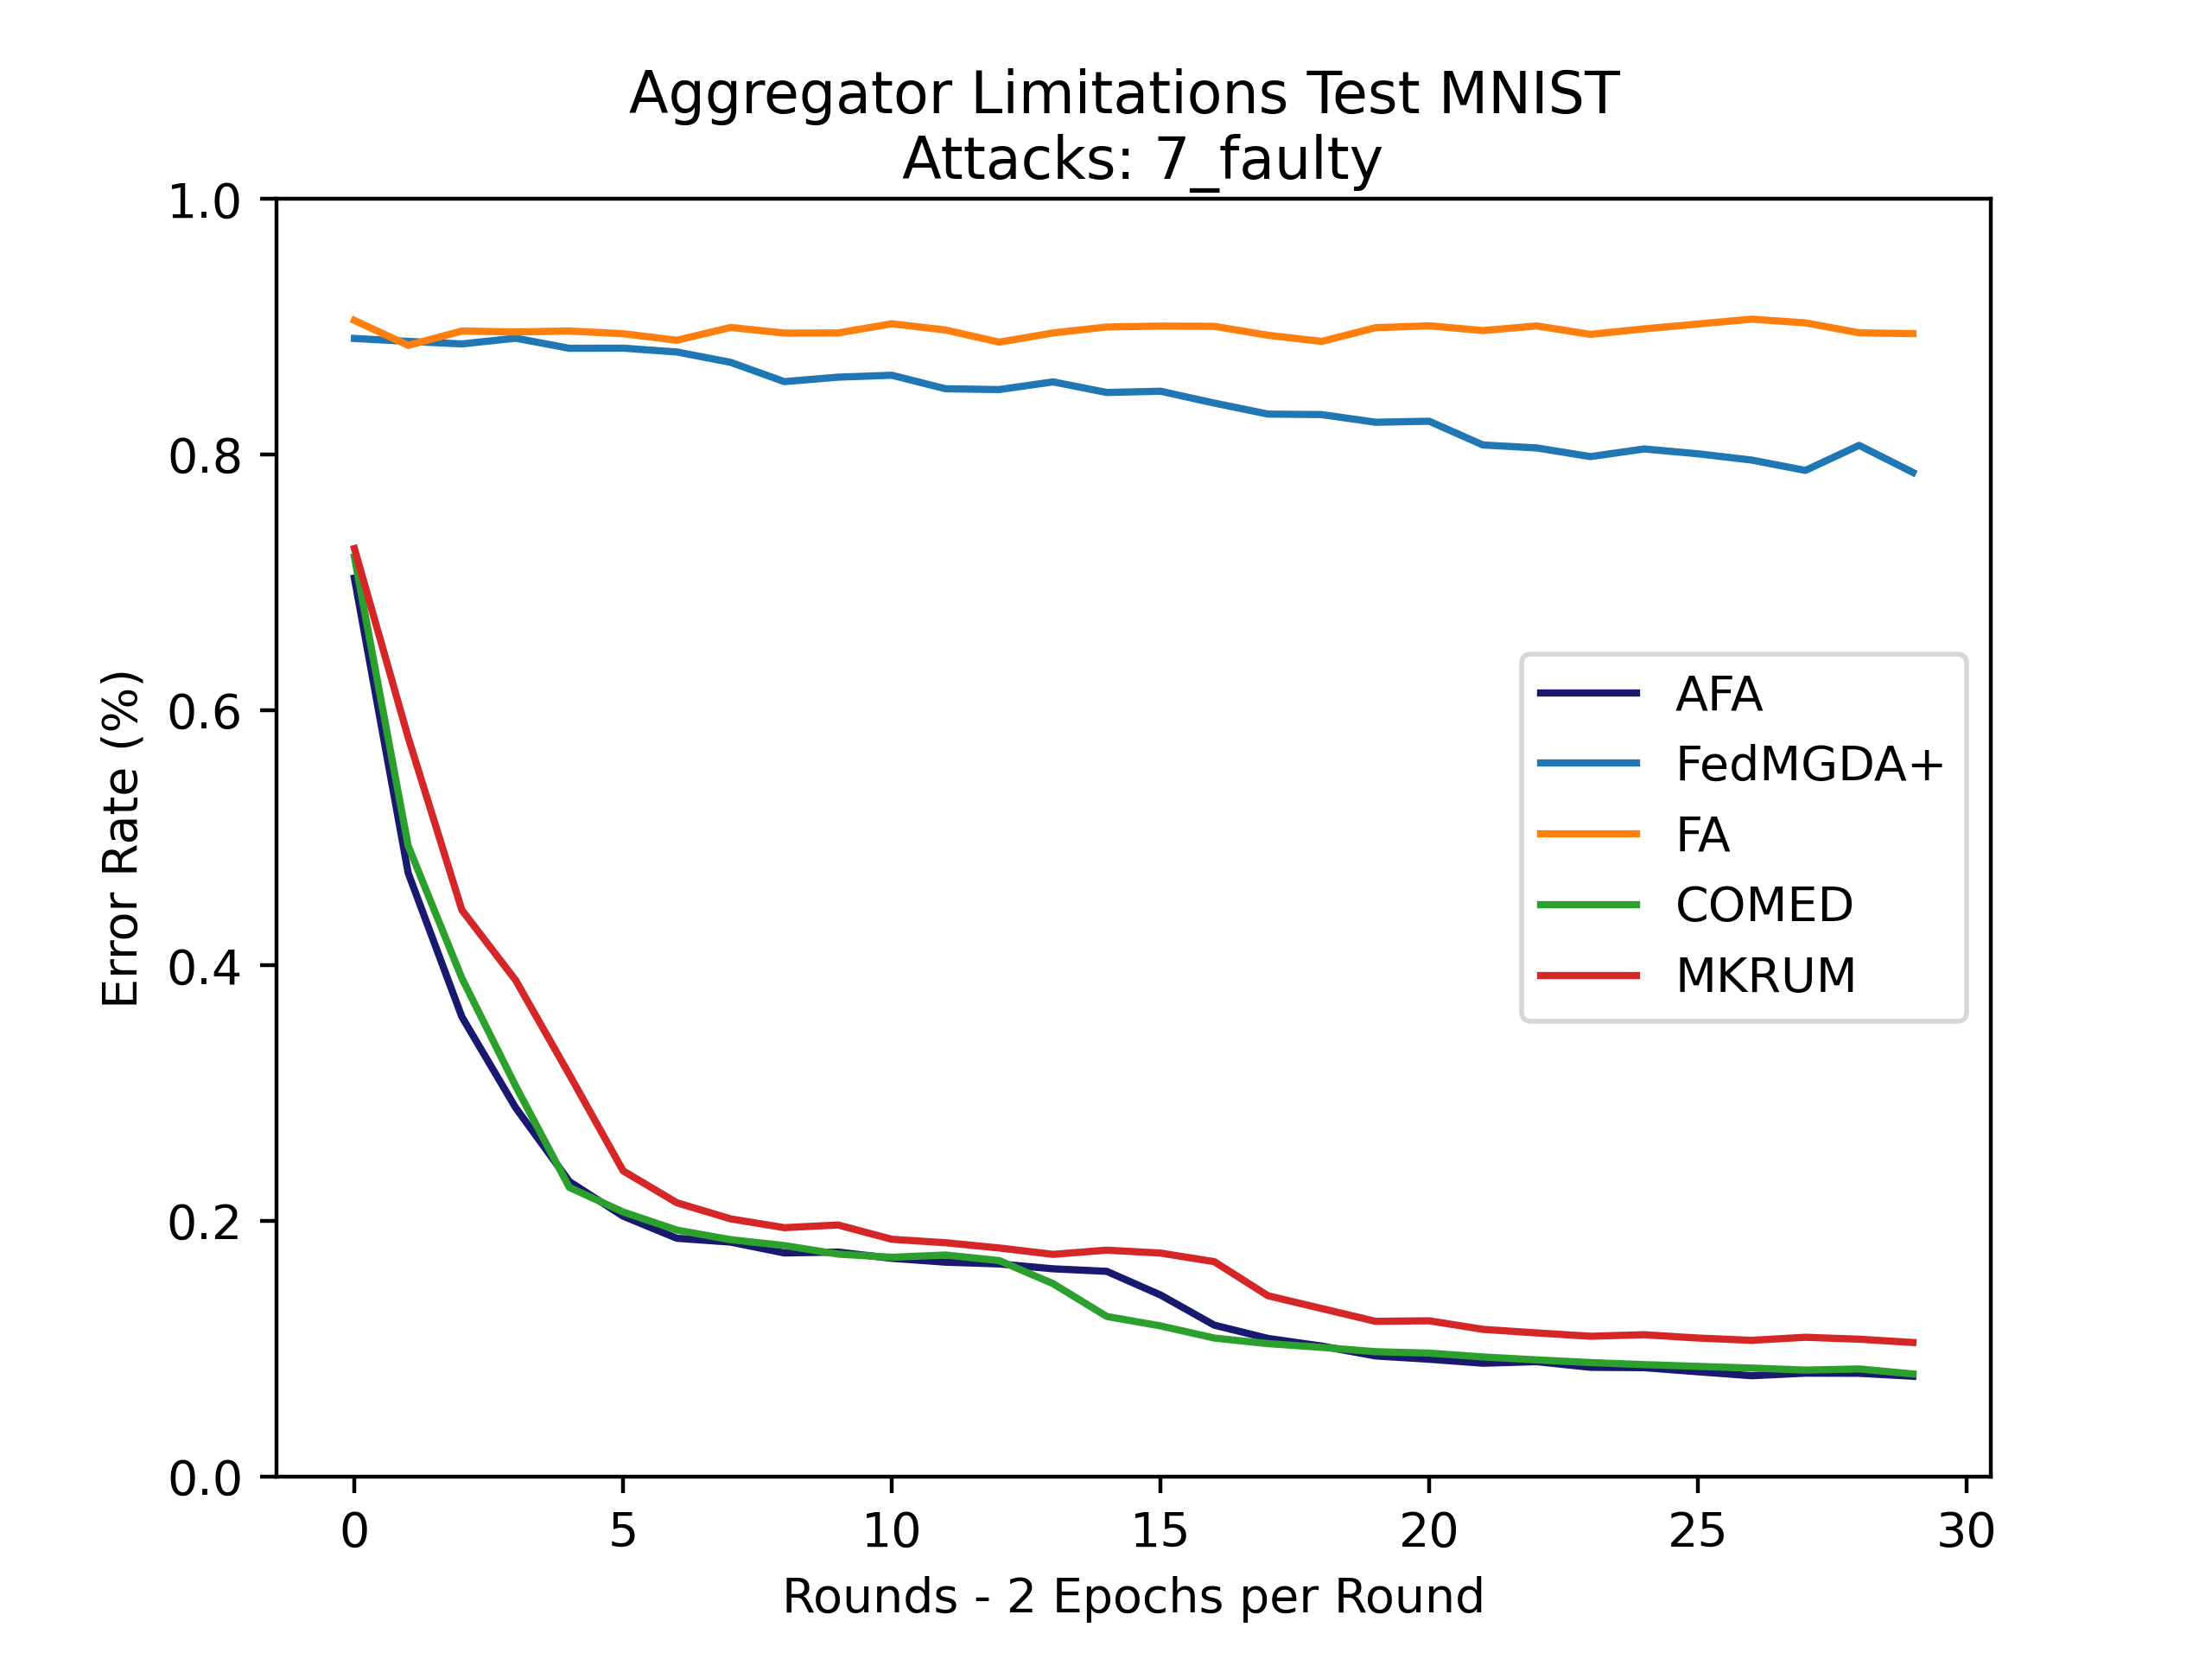
\includegraphics[scale=0.5]{initial/graphs/7_faulty.png}
	\caption{Slow Learning from FedMGDA++}
	\label{fig:7faulty}
\end{figure}

\begin{figure}[htbp]
	\centering
    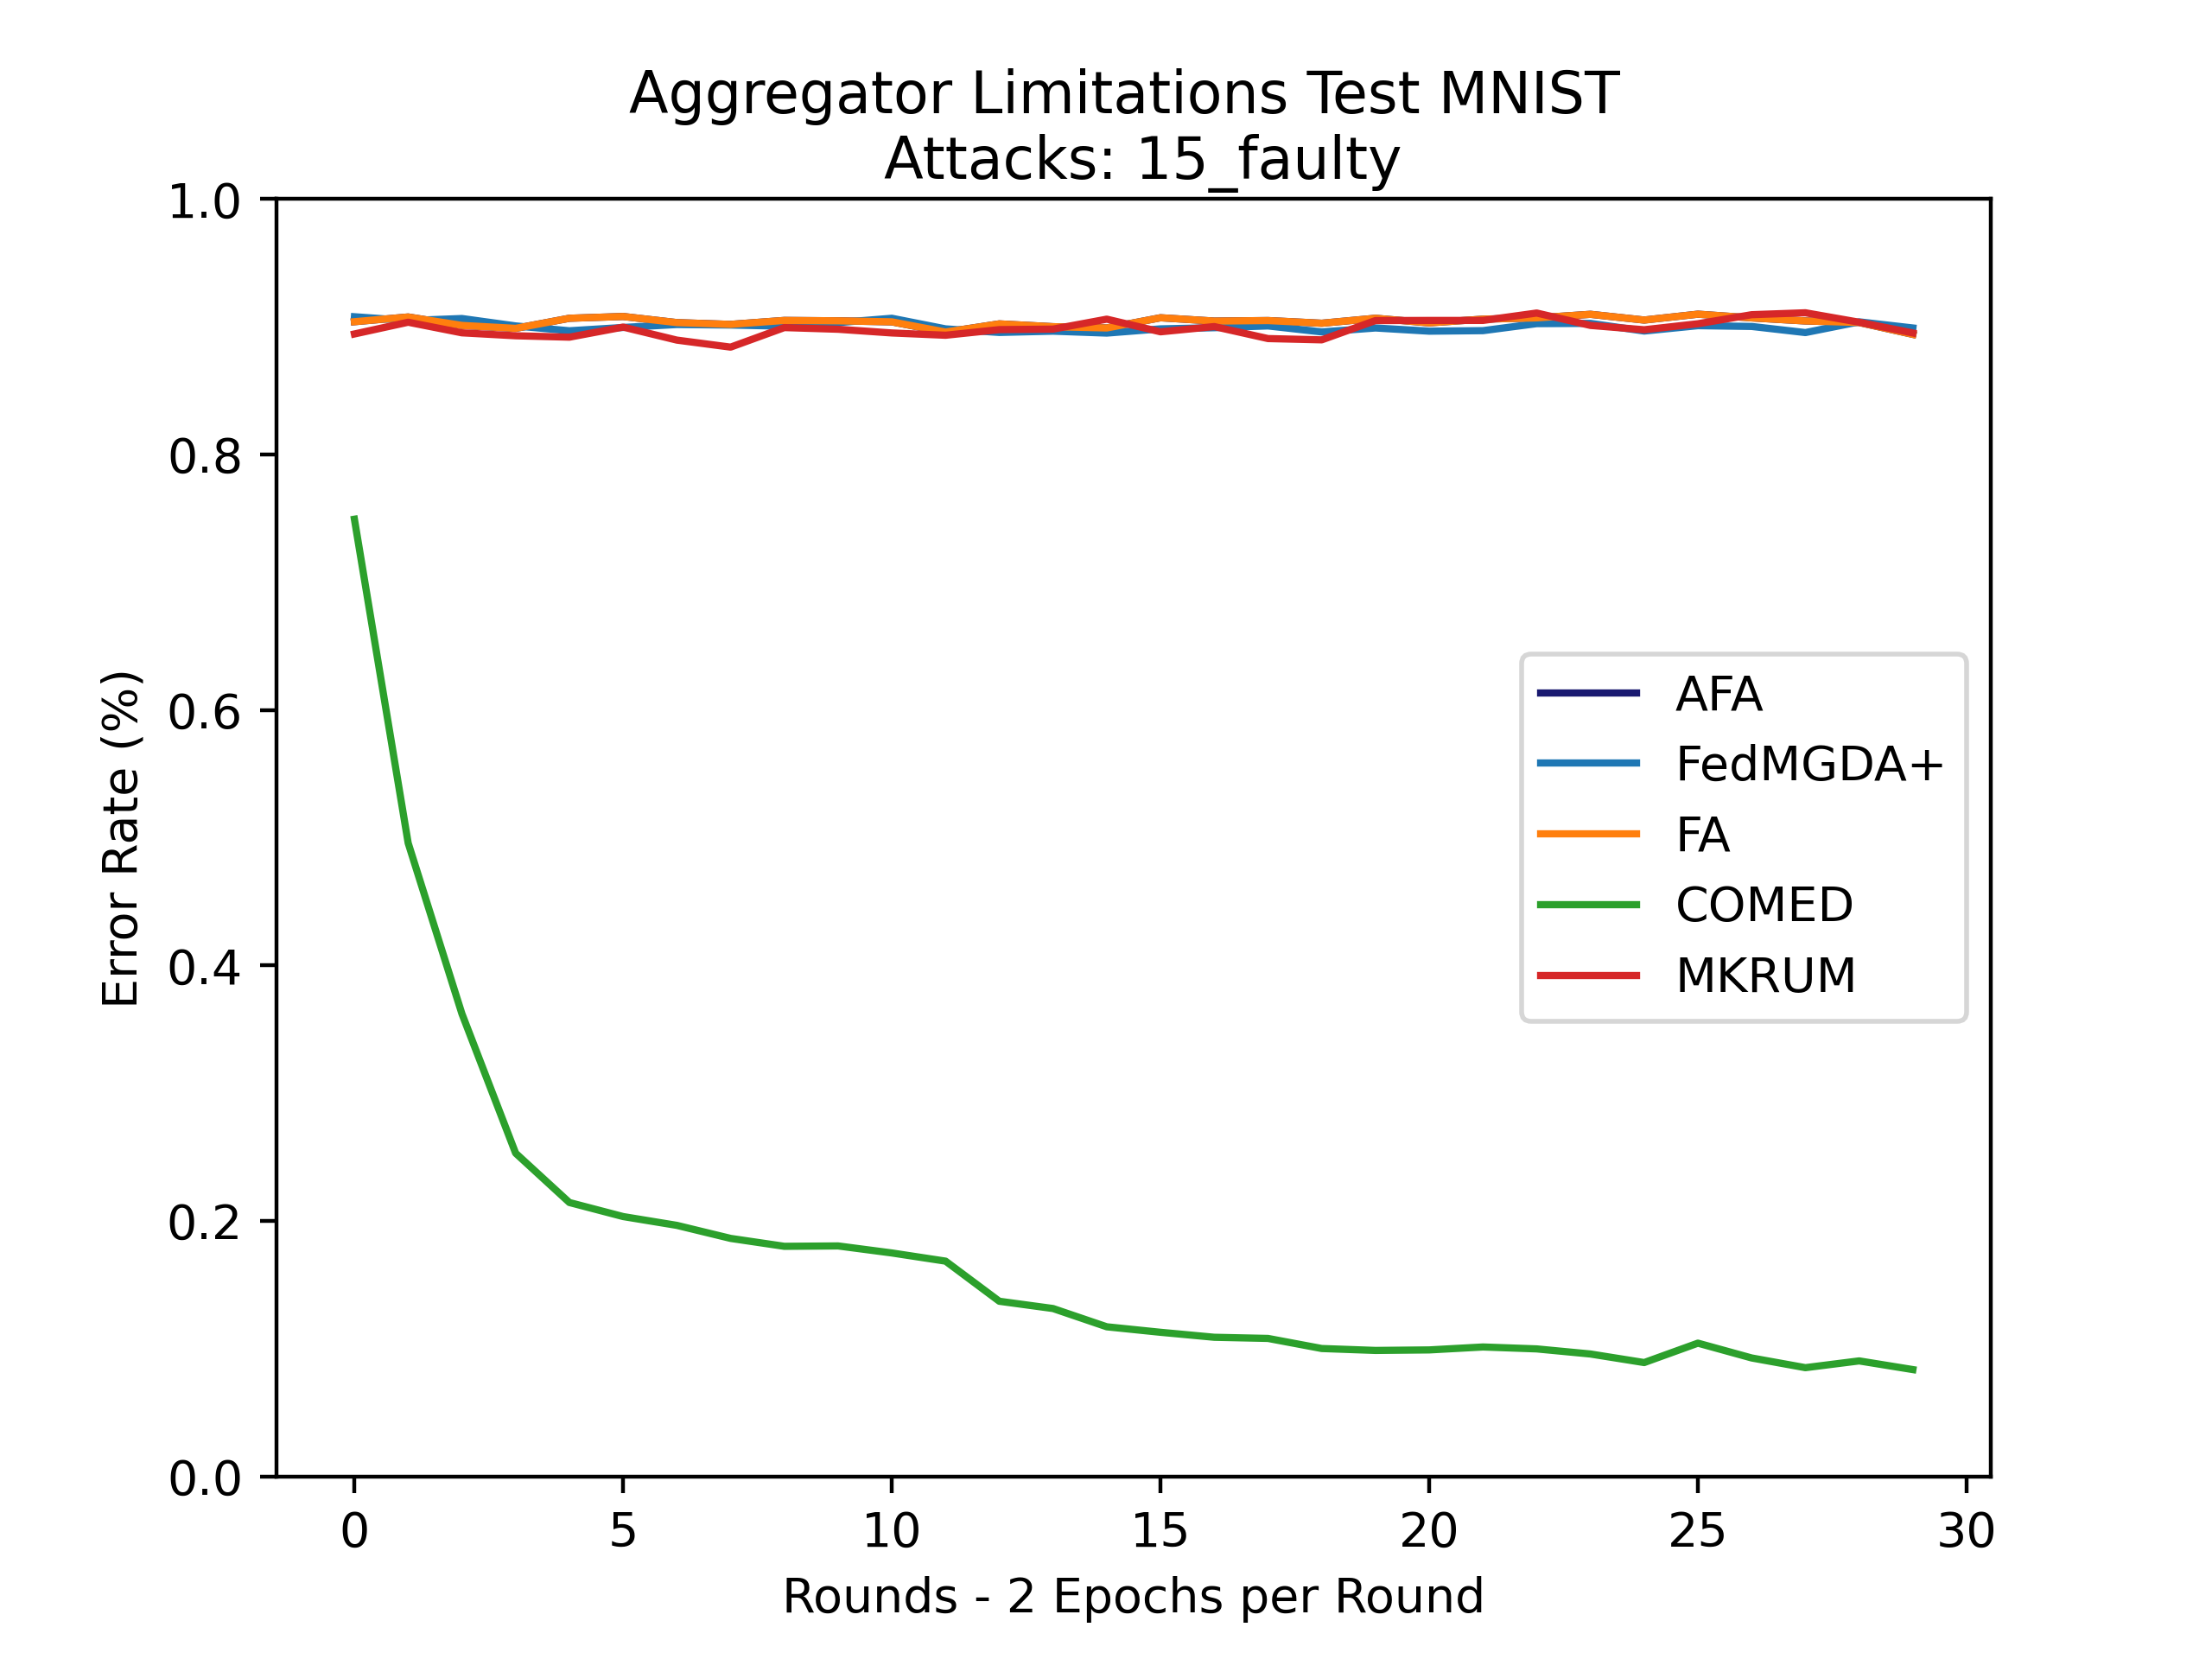
\includegraphics[scale=0.5]{initial/graphs/15_faulty.png}
	\caption{Attempts to Still Learn from Broken Aggregators}
	\label{fig:15faulty}
\end{figure}

